\documentclass[12pt,a4paper]{report}

% ══════════════════════════════════════════════════════════════════
%  PACKAGES
% ══════════════════════════════════════════════════════════════════
\usepackage[utf8]{inputenc}
\usepackage[T1]{fontenc}
\usepackage{times}                    % Times New Roman
\usepackage[english]{babel}
\usepackage{geometry}
\geometry{
  top=2.5cm, bottom=2.5cm,
  left=3cm, right=2.5cm
}
\usepackage{setspace}
\onehalfspacing                       % 1.5 line spacing

\usepackage{graphicx}
\usepackage{float}
\usepackage{caption}
\usepackage{subcaption}
\usepackage{booktabs}
\usepackage{longtable}
\usepackage{array}
\usepackage{tabularx}
\usepackage{multirow}
\usepackage{enumitem}
\usepackage{listings}
\usepackage{xcolor}
\usepackage{hyperref}
\usepackage{url}
\usepackage{fancyhdr}
\usepackage{titlesec}
\usepackage{tocloft}
\usepackage{natbib}
\usepackage{amsmath}
\usepackage{tikz}
\usepackage{pdfpages}
\usepackage{lipsum}

% ── Hyperref settings ───────────────────────────────────────────
\hypersetup{
  colorlinks=true,
  linkcolor=black,
  citecolor=black,
  urlcolor=blue,
  pdftitle={AI-Enhanced Multi-Tenant ERP System},
  pdfauthor={Salah Abdullah Khalil},
}

% ── Code listing style ──────────────────────────────────────────
\definecolor{codebg}{rgb}{0.95,0.95,0.95}
\definecolor{codegreen}{rgb}{0,0.5,0}
\definecolor{codegray}{rgb}{0.5,0.5,0.5}
\definecolor{codepurple}{rgb}{0.58,0,0.82}

\lstdefinestyle{pythonstyle}{
  backgroundcolor=\color{codebg},
  commentstyle=\color{codegreen},
  keywordstyle=\color{codepurple}\bfseries,
  stringstyle=\color{orange},
  basicstyle=\ttfamily\footnotesize,
  breaklines=true,
  frame=single,
  numbers=left,
  numberstyle=\tiny\color{codegray},
  tabsize=4,
  language=Python,
  showstringspaces=false,
}
\lstset{style=pythonstyle}

% ── Header/Footer ──────────────────────────────────────────────
\pagestyle{fancy}
\fancyhf{}
\fancyhead[R]{\leftmark}
\fancyfoot[C]{\thepage}
\renewcommand{\headrulewidth}{0.4pt}

% ── Chapter/Section formatting ─────────────────────────────────
\titleformat{\chapter}[display]
  {\normalfont\huge\bfseries\centering}
  {\chaptertitlename\ \thechapter}{20pt}{\Huge}
\titlespacing*{\chapter}{0pt}{-30pt}{40pt}

% ── Placeholder image command ──────────────────────────────────
\newcommand{\placeholderimg}[2][0.8]{%
  \begin{figure}[H]
    \centering
    \fbox{\parbox{#1\textwidth}{\vspace{4cm}\centering\large\textit{#2}\vspace{4cm}}}
  \end{figure}
}

\newcommand{\placeholderimgcap}[3][0.8]{%
  \begin{figure}[H]
    \centering
    \fbox{\parbox{#1\textwidth}{\vspace{3.5cm}\centering\large\textit{#2}\vspace{3.5cm}}}
    \caption{#3}
    \label{fig:#2}
  \end{figure}
}


% ══════════════════════════════════════════════════════════════════
%  DOCUMENT BEGIN
% ══════════════════════════════════════════════════════════════════
\begin{document}

% ══════════════════════════════════════════════════════════════════
%  COVER PAGE
% ══════════════════════════════════════════════════════════════════
\begin{titlepage}
\begin{center}

\vspace*{0.5cm}

% ── University Logo Placeholder ─────────────────────────────────
\fbox{\parbox{4cm}{\vspace{2cm}\centering\textit{University Logo}\vspace{2cm}}}

\vspace{1cm}

{\Large\textbf{Kingdom of Saudi Arabia}}\\[0.3cm]
{\Large\textbf{Ministry of Education}}\\[0.3cm]
{\Large\textbf{University Name}}\\[0.3cm]
{\large\textbf{College of Computer Science and Information Technology}}\\[0.3cm]
{\large\textbf{Department of Information Technology}}\\[1.5cm]

{\LARGE\textbf{Design and Implementation of an AI-Enhanced\\[0.3cm]
Multi-Tenant Enterprise Resource Planning System\\[0.3cm]
Using Machine Learning for Business Intelligence}}\\[2cm]

{\large A Graduation Project Submitted in Partial Fulfillment of the\\
Requirements for the Degree of\\[0.3cm]
\textbf{Bachelor of Science in Information Technology}}\\[1.5cm]

{\large\textbf{Prepared by:}}\\[0.3cm]
{\large Salah Abdullah Khalil}\\[1cm]

{\large\textbf{Supervised by:}}\\[0.3cm]
{\large [Supervisor Name]}\\[1.5cm]

{\large\textbf{First Semester 1447 / 2025--2026}}

\end{center}
\end{titlepage}

% ══════════════════════════════════════════════════════════════════
%  BISMILLAH PAGE
% ══════════════════════════════════════════════════════════════════
\newpage
\thispagestyle{empty}
\vspace*{\fill}
\begin{center}
{\Huge\textit{In the Name of Allah, the Most Gracious, the Most Merciful}}
\end{center}
\vspace*{\fill}
\newpage

% ══════════════════════════════════════════════════════════════════
%  DEDICATION
% ══════════════════════════════════════════════════════════════════
\newpage
\thispagestyle{empty}
\vspace*{3cm}
\begin{center}
{\LARGE\textbf{Dedication}}\\[1.5cm]
\end{center}

\begin{quote}
\large
\textit{I dedicate this work to my beloved parents, whose unwavering support and encouragement have been my greatest source of strength throughout my academic journey. To my family and friends who have stood by me with patience and understanding. And to all those who believe in the power of technology to transform businesses and create a better future.}
\end{quote}
\newpage

% ══════════════════════════════════════════════════════════════════
%  ACKNOWLEDGMENTS
% ══════════════════════════════════════════════════════════════════
\newpage
\thispagestyle{empty}
\vspace*{2cm}
\begin{center}
{\LARGE\textbf{Acknowledgments}}\\[1.5cm]
\end{center}

First and foremost, I thank \textbf{Allah (SWT)} for granting me the strength, knowledge, and perseverance to complete this graduation project.

I would like to express my sincere gratitude to my supervisor, \textbf{[Supervisor Name]}, for the continuous guidance, valuable feedback, and encouragement throughout this research. Your expertise and mentorship have been instrumental in shaping this work.

I am deeply grateful to the \textbf{Faculty of Computer Science and Information Technology} at \textbf{[University Name]} for providing an enriching academic environment and the resources necessary to undertake this project.

Special thanks to my colleagues and friends who provided constructive criticism, participated in testing, and offered their insights during the development process.

Finally, I extend my heartfelt appreciation to my \textbf{family}, especially my parents, for their unconditional love, support, and prayers that have carried me through every challenge.

\newpage

% ══════════════════════════════════════════════════════════════════
%  ABSTRACT
% ══════════════════════════════════════════════════════════════════
\newpage
\thispagestyle{empty}
\vspace*{2cm}
\begin{center}
{\LARGE\textbf{Abstract}}\\[1.5cm]
\end{center}

Enterprise Resource Planning (ERP) systems serve as the backbone of modern organizational management by integrating core business processes into a unified platform. However, small and medium enterprises (SMEs) in the Middle East and North Africa (MENA) region face significant barriers to adopting commercial ERP solutions, including prohibitive licensing costs, lack of Arabic language support, and limited customization capabilities. Furthermore, traditional ERP systems largely function as passive record-keeping tools, lacking the predictive and prescriptive intelligence required for proactive business decision-making.

This graduation project presents the design and implementation of an \textbf{AI-Enhanced Multi-Tenant ERP System} built on the Django web framework with PostgreSQL database isolation per tenant. The system integrates \textbf{eight machine learning models} spanning five business domains: (1)~Lead Scoring using Logistic Regression, (2)~Late Payment Prediction using Gradient Boosted Trees, (3)~Employee Attrition Risk using Random Forest, (4)~Expense Anomaly Detection using Isolation Forest, (5)~Attendance Pattern Analysis using Z-Score statistics, (6)~Demand Forecasting using Facebook Prophet, (7)~Cash Flow Projection using rule-based modeling, and (8)~KPI Anomaly Detection using statistical process control.

The system was developed following the \textbf{Sprint (Agile)} methodology with iterative development cycles. The architecture features over 80 domain models organized into nine functional modules (Finance, HR, CRM, Inventory/WMS, POS, Fixed Assets, Suppliers, Reporting, and AI), a complete REST API, and a real-time AI Insight notification engine. Multi-tenancy is achieved through dynamic PostgreSQL database provisioning via Docker containers or remote server connections, ensuring complete data isolation between organizations.

Experimental evaluation demonstrates strong model performance: Late Payment Prediction achieves an AUC-ROC of \textbf{0.9867}, Employee Attrition Prediction achieves \textbf{0.9475}, Demand Forecasting achieves an average accuracy of \textbf{0.7249} across 80 products using Prophet cross-validation, and the KPI Anomaly Detector successfully identifies statistically significant business metric deviations with calibrated z-score thresholds.

\vspace{0.5cm}
\noindent\textbf{Keywords:} ERP System, Machine Learning, Multi-Tenant Architecture, Django, Business Intelligence, Demand Forecasting, Anomaly Detection, Prophet, Gradient Boosting, Agile Development.

\newpage

% ══════════════════════════════════════════════════════════════════
%  TABLE OF CONTENTS
% ══════════════════════════════════════════════════════════════════
\pagenumbering{roman}
\tableofcontents
\newpage
\listoffigures
\newpage
\listoftables
\newpage

% ══════════════════════════════════════════════════════════════════
%  LIST OF ABBREVIATIONS
% ══════════════════════════════════════════════════════════════════
\chapter*{List of Abbreviations}
\addcontentsline{toc}{chapter}{List of Abbreviations}

\begin{longtable}{@{} l p{10cm} @{}}
\toprule
\textbf{Abbreviation} & \textbf{Full Term} \\
\midrule
\endfirsthead
\toprule
\textbf{Abbreviation} & \textbf{Full Term} \\
\midrule
\endhead
AI      & Artificial Intelligence \\
API     & Application Programming Interface \\
AUC     & Area Under the Curve \\
CRM     & Customer Relationship Management \\
CRUD    & Create, Read, Update, Delete \\
CSV     & Comma-Separated Values \\
DRF     & Django REST Framework \\
ERP     & Enterprise Resource Planning \\
FK      & Foreign Key \\
GBM     & Gradient Boosting Machine \\
HR      & Human Resources \\
JSON    & JavaScript Object Notation \\
KPI     & Key Performance Indicator \\
MAE     & Mean Absolute Error \\
MENA    & Middle East and North Africa \\
ML      & Machine Learning \\
ORM     & Object-Relational Mapping \\
PO      & Purchase Order \\
POS     & Point of Sale \\
REST    & Representational State Transfer \\
ROC     & Receiver Operating Characteristic \\
SME     & Small and Medium Enterprise \\
SQL     & Structured Query Language \\
UI      & User Interface \\
UUID    & Universally Unique Identifier \\
WMS     & Warehouse Management System \\
\bottomrule
\end{longtable}

\newpage
\pagenumbering{arabic}
\setcounter{page}{1}

% ██████████████████████████████████████████████████████████████████
%
%  CHAPTER 1 — INTRODUCTION
%
% ██████████████████████████████████████████████████████████████████
\chapter{Introduction}
\label{ch:introduction}

\section{Overview}
\label{sec:overview}

Enterprise Resource Planning (ERP) systems have become indispensable tools for organizations seeking to integrate and streamline their core business processes. An ERP system consolidates diverse functional areas---including finance, human resources, customer relationship management, inventory, and procurement---into a single unified platform that facilitates data sharing, eliminates redundancy, and enables informed decision-making \citep{monk2013concepts}. The global ERP market was valued at approximately USD 54.76 billion in 2022 and is projected to reach USD 123.41 billion by 2030, reflecting the growing recognition of ERP as a strategic asset rather than a mere operational tool \citep{grandviewresearch2023}.

Despite this growth, the adoption of ERP systems among small and medium enterprises (SMEs) in the Middle East and North Africa (MENA) region remains disproportionately low compared to markets in North America and Europe. Research indicates that key barriers include the high total cost of ownership of commercial solutions such as SAP and Oracle, the scarcity of Arabic language support in open-source alternatives, the complexity of deployment and customization, and the limited IT infrastructure in many SMEs \citep{almajali2016antecedents}. These challenges leave a substantial segment of the business landscape relying on disconnected spreadsheets, manual processes, and fragmented software tools that hinder growth and competitiveness.

Concurrently, the rapid advancement of Artificial Intelligence (AI) and Machine Learning (ML) has opened new opportunities for augmenting traditional business systems with predictive and prescriptive capabilities. Modern ML algorithms can analyze historical business data to forecast demand, predict customer payment behavior, detect anomalies in financial transactions, and identify employees at risk of attrition---capabilities that transform an ERP system from a passive record-keeper into a proactive decision-support platform \citep{davenport2018ai}.

This project addresses both challenges simultaneously by designing and implementing an \textbf{AI-Enhanced Multi-Tenant ERP System} that is (a)~accessible and affordable for SMEs through a multi-tenant Software-as-a-Service (SaaS) architecture, (b)~built with Arabic language support from the ground up, and (c)~integrated with eight machine learning models that provide actionable business intelligence across five functional domains.

\section{Problem Statement}
\label{sec:problem_statement}

The current landscape of ERP adoption among SMEs, particularly in the MENA region, is characterized by several interconnected problems:

\begin{enumerate}[label=\arabic*.]
  \item \textbf{High Cost of Commercial ERP Solutions:} Leading ERP systems such as SAP Business One, Oracle NetSuite, and Microsoft Dynamics 365 impose substantial licensing fees, implementation costs, and ongoing maintenance expenses that place them beyond the reach of most SMEs. A Panorama Consulting Group survey found that the average ERP implementation cost exceeds USD 170,000 for small organizations \citep{panorama2023}.

  \item \textbf{Limited Arabic Language Support:} Most open-source ERP platforms (e.g., Odoo Community, ERPNext) provide only partial or community-contributed Arabic translations. Critical modules such as financial reporting, tax compliance, and user interfaces often lack proper right-to-left (RTL) rendering and cultural localization \citep{alkraiji2020}.

  \item \textbf{Absence of Integrated AI Capabilities:} Traditional ERP systems are designed primarily for recording and reporting historical transactions. They do not incorporate predictive analytics, anomaly detection, or intelligent forecasting within their core workflows. Organizations seeking these capabilities must invest in separate Business Intelligence (BI) tools and custom integrations, increasing both cost and complexity \citep{lee2020erp}.

  \item \textbf{Rigid Single-Tenant Architectures:} Many existing ERP solutions follow a single-tenant deployment model that requires dedicated infrastructure for each organization, driving up hosting costs and administrative overhead. Multi-tenant architectures, which allow multiple organizations to share the same application instance while maintaining complete data isolation, are more cost-effective but technically challenging to implement correctly \citep{bezemer2010multi}.

  \item \textbf{Lack of Proactive Decision Support:} Business managers frequently make critical decisions---such as inventory reorder quantities, credit terms, employee retention strategies, and cash flow management---based on intuition rather than data-driven insights. The absence of embedded ML models within the ERP workflow means that valuable predictive signals buried in transactional data remain unexploited \citep{provost2013data}.
\end{enumerate}

\section{Project Objectives}
\label{sec:objectives}

This project aims to achieve the following objectives:

\begin{enumerate}[label=\arabic*.]
  \item Design and implement a comprehensive, web-based ERP system covering nine functional modules: Finance, Human Resources, Customer Relationship Management (CRM), Inventory and Warehouse Management, Supplier and Procurement, Point of Sale (POS), Fixed Assets, Reporting, and Artificial Intelligence.

  \item Implement a robust multi-tenant architecture using database-per-tenant isolation with dynamic PostgreSQL database provisioning via Docker containers and remote server connections.

  \item Integrate eight machine learning models into the ERP workflow:
  \begin{itemize}
    \item \textit{Lead Scoring} --- Logistic Regression for CRM conversion prediction
    \item \textit{Late Payment Prediction} --- Gradient Boosted Trees for accounts receivable risk
    \item \textit{Employee Attrition Risk} --- Random Forest for HR retention planning
    \item \textit{Expense Anomaly Detection} --- Isolation Forest for fraud and policy violation identification
    \item \textit{Attendance Anomaly Detection} --- Z-Score analysis for workforce pattern recognition
    \item \textit{Demand Forecasting} --- Facebook Prophet for inventory reorder optimization
    \item \textit{Cash Flow Projection} --- Rule-based modeling for financial planning
    \item \textit{KPI Anomaly Detection} --- Statistical process control for business metric monitoring
  \end{itemize}

  \item Develop an AI Insight Engine that automatically generates actionable alerts and recommendations from ML model outputs and delivers them as real-time notifications to relevant users.

  \item Provide bilingual support (English and Arabic) with proper RTL rendering throughout the user interface.

  \item Follow the Sprint (Agile) software development methodology to ensure iterative delivery, continuous testing, and stakeholder feedback incorporation.
\end{enumerate}

\section{Project Scope}
\label{sec:scope}

The scope of this project encompasses the following:

\subsection{In Scope}
\begin{itemize}
  \item Full-stack web application development using Django 4.2 (Python) as the backend framework.
  \item PostgreSQL as the relational database management system for both the main (platform) database and all tenant databases.
  \item Multi-tenant platform administration: user signup, approval workflow, database provisioning, and role-based access control (Owner, Admin, User, Read-Only).
  \item Nine ERP functional modules with complete CRUD operations, business logic, and reporting.
  \item Eight ML models with training pipelines, model versioning, prediction logging, and accuracy evaluation.
  \item RESTful API layer using Django REST Framework (DRF) for mobile and third-party integration.
  \item AI Insight notification system with severity levels (Info, Warning, Critical) and automatic deduplication.
  \item Asynchronous task processing using Celery with Redis as the message broker.
  \item Data seeding utilities for testing and demonstration.
\end{itemize}

\subsection{Out of Scope}
\begin{itemize}
  \item Native mobile application development (the system is accessible via mobile browsers and a REST API is provided for future native app development).
  \item Integration with external accounting authorities or government e-invoicing APIs (e.g., ZATCA in Saudi Arabia).
  \item Deep learning models (CNN, RNN, Transformers) for natural language processing or image recognition---the AI scope is limited to classical ML and time-series forecasting.
  \item Load testing and performance benchmarking for production-scale deployments.
\end{itemize}

\section{Project Significance}
\label{sec:significance}

This project makes several contributions:

\begin{enumerate}[label=\arabic*.]
  \item \textbf{Practical Contribution:} It delivers a fully functional, production-ready ERP system that SMEs in the MENA region can deploy without the licensing costs associated with commercial alternatives. The multi-tenant SaaS model further reduces per-organization costs by sharing infrastructure.

  \item \textbf{Technical Innovation:} To the best of our knowledge, this is among the first open-source ERP implementations that embeds eight ML models directly within the transactional workflow---not as an external BI layer, but as integral components that train on the organization's own data, generate predictions in real time, and write actionable insights back into the ERP.

  \item \textbf{Academic Contribution:} The project demonstrates the practical application of multiple ML algorithms (Logistic Regression, Gradient Boosting, Random Forest, Isolation Forest, Prophet, Z-Score) to real-world ERP datasets, providing empirical performance metrics (AUC-ROC, MAE, F1-Score) that contribute to the body of knowledge on applied machine learning in business systems.

  \item \textbf{Bilingual Accessibility:} By incorporating Arabic names, labels, and RTL support at the model level (dual-language fields throughout all 80+ models), the system addresses a persistent localization gap in open-source ERP solutions.
\end{enumerate}

\section{Project Questions}
\label{sec:questions}

This project seeks to answer the following research questions:

\begin{enumerate}[label=\textbf{RQ\arabic*:}]
  \item How can a multi-tenant ERP system with database-per-tenant isolation be effectively designed and implemented using Django and PostgreSQL to achieve both data security and cost efficiency?

  \item To what extent can machine learning models trained on ERP transactional data provide accurate and actionable predictions for business processes such as demand forecasting, payment risk assessment, and employee attrition?

  \item What software architecture and design patterns are required to seamlessly integrate ML model training, prediction, and insight generation into the standard ERP operational workflow?

  \item How does the Sprint (Agile) development methodology facilitate the iterative development of a complex, multi-module ERP system with integrated AI capabilities?
\end{enumerate}

\section{Report Organization}
\label{sec:organization}

The remainder of this report is organized as follows:

\begin{itemize}
  \item \textbf{Chapter 2 --- Literature Review:} Provides a comprehensive review of existing ERP systems, multi-tenant architectures, and the application of machine learning in enterprise systems. It examines related work and identifies the gaps that this project addresses.

  \item \textbf{Chapter 3 --- Methodology:} Describes the Sprint (Agile) development methodology adopted, the system architecture, the technology stack, and the ML model design and evaluation approach.

  \item \textbf{Chapter 4 --- System Analysis and Design:} Presents the system requirements (functional and non-functional), use case diagrams, class diagrams, database schema design, and the AI/ML pipeline architecture.

  \item \textbf{Chapter 5 --- Implementation and Testing:} Details the implementation of key system components, code structure, ML model training results, and testing procedures.

  \item \textbf{Chapter 6 --- Results and Discussion:} Analyzes the ML model performance metrics, system usability, and discusses the findings in the context of the research questions.

  \item \textbf{Chapter 7 --- Conclusion and Future Work:} Summarizes the contributions, acknowledges limitations, and proposes directions for future enhancement.
\end{itemize}


% ██████████████████████████████████████████████████████████████████
%
%  CHAPTER 2 — LITERATURE REVIEW
%
% ██████████████████████████████████████████████████████████████████
\chapter{Literature Review}
\label{ch:literature_review}

\section{Introduction}
\label{sec:lit_intro}

This chapter provides a comprehensive review of the theoretical foundations and existing work relevant to the three core pillars of this project: Enterprise Resource Planning systems, multi-tenant software architectures, and the application of machine learning in business systems. The review establishes the academic context, identifies gaps in current solutions, and justifies the design decisions adopted in this project.

\section{Enterprise Resource Planning (ERP) Systems}
\label{sec:erp_systems}

\subsection{Definition and Evolution}

Enterprise Resource Planning (ERP) is defined as an integrated software system that manages and automates core business processes across an organization through a shared database and standardized workflows \citep{monk2013concepts}. The evolution of ERP systems can be traced through three generations:

\begin{enumerate}[label=\arabic*.]
  \item \textbf{Material Requirements Planning (MRP), 1970s:} Focused exclusively on manufacturing---calculating raw material needs based on production schedules and bills of materials. IBM's COPICS and SAP R/1 were early examples \citep{jacobs2007enterprise}.

  \item \textbf{MRP II and Early ERP, 1980s--1990s:} Extended MRP to include finance, HR, and distribution. SAP R/3, introduced in 1992, pioneered the client-server ERP model with real-time integration across modules \citep{jacobs2007enterprise}. This era established the ``ERP'' terminology and saw rapid adoption by large enterprises.

  \item \textbf{Modern Cloud ERP, 2010s--Present:} The shift to web-based, cloud-hosted architectures has democratized ERP access. Solutions like SAP S/4HANA Cloud, Oracle NetSuite, and open-source platforms such as Odoo and ERPNext enable SaaS deployment models that reduce upfront investment \citep{panorama2023}.
\end{enumerate}

\begin{figure}[H]
    \centering
    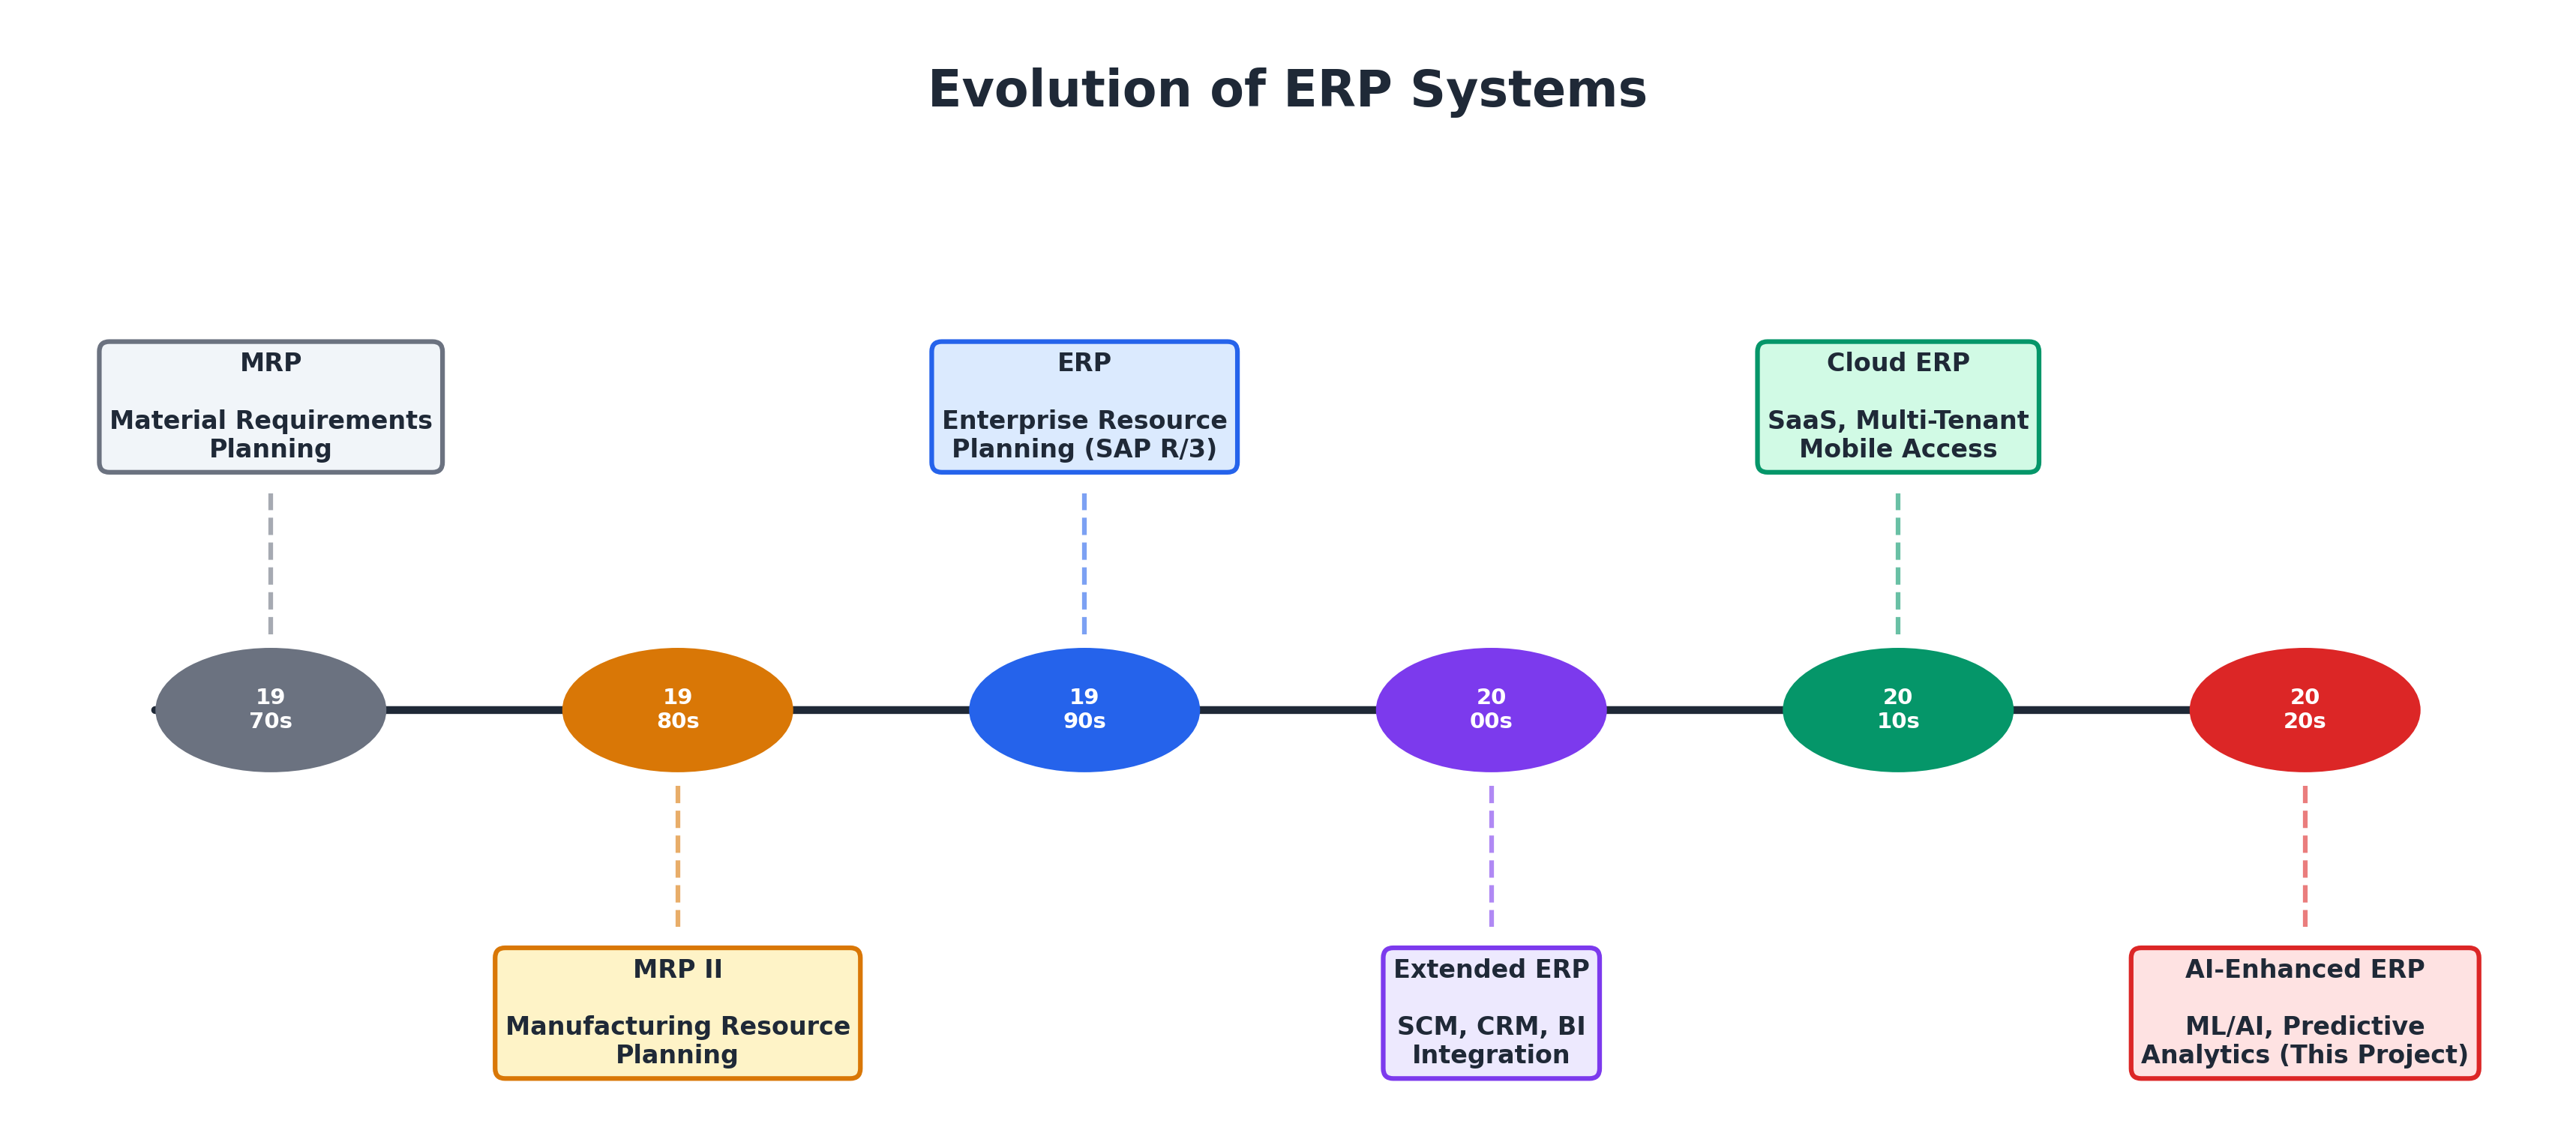
\includegraphics[width=0.95\textwidth]{figures/erp_evolution_timeline.png}
    \caption{Evolution of ERP systems from MRP (1970s) to Cloud AI-ERP (2020s)}
    \label{fig:erp_evolution}
\end{figure}

\subsection{ERP Architecture Models}

Modern ERP systems are typically deployed using one of three architectural models:

\begin{itemize}
  \item \textbf{Monolithic Architecture:} All modules are packaged as a single deployable unit sharing one database. Traditional SAP R/3 and Oracle E-Business Suite follow this model. While simple to deploy, monolithic architectures are difficult to scale and customize \citep{bezemer2010multi}.

  \item \textbf{Service-Oriented Architecture (SOA):} Business functions are decomposed into loosely coupled services that communicate via standardized protocols. Modern SAP S/4HANA adopts elements of SOA to enable extensibility \citep{krafzig2005enterprise}.

  \item \textbf{Microservices Architecture:} An evolution of SOA where each service is independently deployable and scalable. While offering maximum flexibility, this model introduces operational complexity that makes it less suitable for SME-focused projects \citep{newman2015building}.
\end{itemize}

This project adopts a \textbf{modular monolith} architecture---a single Django application with clearly separated modules (apps) that share a common codebase but maintain logical boundaries. This balances simplicity with maintainability and is well-suited for the project scope.

\subsection{ERP Adoption in SMEs}

Research by \citet{almajali2016antecedents} identifies organizational factors (top management support, organizational readiness), technological factors (system complexity, compatibility), and environmental factors (competitive pressure, vendor support) as determinants of ERP adoption success in Jordanian SMEs. Their findings highlight that \textit{perceived cost} and \textit{organizational readiness} are the strongest predictors of adoption intent.

A study by \citet{panorama2023} found that among organizations implementing ERP, 50\% reported exceeding their initial budget, and the average implementation timeline for SMEs was 14.3 months. These statistics underscore the need for lightweight, rapid-deployment ERP solutions---a gap this project addresses through its Django-based architecture and Sprint development methodology.

\subsection{Open-Source ERP Systems}

Several open-source ERP platforms have emerged as alternatives to commercial solutions:

\begin{table}[H]
\centering
\caption{Comparison of major open-source ERP systems}
\label{tab:erp_comparison}
\begin{tabularx}{\textwidth}{l X X X X}
\toprule
\textbf{Feature} & \textbf{Odoo CE} & \textbf{ERPNext} & \textbf{Dolibarr} & \textbf{This Project} \\
\midrule
Language & Python & Python/JS & PHP & Python (Django) \\
Database & PostgreSQL & MariaDB & MySQL/PgSQL & PostgreSQL \\
Multi-Tenant & Limited & No & No & \textbf{Yes (DB-per-tenant)} \\
Arabic Support & Partial & Partial & Minimal & \textbf{Full (dual fields)} \\
Integrated ML/AI & No & No & No & \textbf{8 ML models} \\
REST API & Yes & Yes & Limited & Yes (DRF) \\
WMS & Enterprise only & Basic & No & \textbf{Full WMS} \\
POS & Enterprise only & Basic & No & \textbf{Yes} \\
License & LGPL v3 & GPL v3 & GPL v3 & -- \\
\bottomrule
\end{tabularx}
\end{table}

As Table~\ref{tab:erp_comparison} illustrates, none of the existing open-source ERP systems combine native multi-tenant isolation, comprehensive Arabic support, and integrated machine learning capabilities---the three distinguishing features of this project.


\section{Multi-Tenant Software Architecture}
\label{sec:multi_tenant}

\subsection{Definition and Models}

Multi-tenancy is a software architecture principle in which a single instance of a software application serves multiple customers (tenants), each of whom perceives the application as if it were running exclusively for them \citep{bezemer2010multi}. Three principal models of multi-tenancy exist:

\begin{enumerate}[label=\arabic*.]
  \item \textbf{Shared Database, Shared Schema:} All tenants share the same database and tables, with a \texttt{tenant\_id} column used to filter data. This is the most resource-efficient model but offers the weakest data isolation and complicates compliance with data sovereignty regulations \citep{chong2006multi}.

  \item \textbf{Shared Database, Separate Schema:} Each tenant has its own database schema (namespace) within a shared database instance. This provides moderate isolation with lower overhead than full database separation. PostgreSQL's native schema support makes this model practical \citep{bezemer2010multi}.

  \item \textbf{Separate Database (Database-per-Tenant):} Each tenant is assigned a dedicated database instance. This model provides the strongest isolation---tenant data is physically separated, simplifying backup, migration, and regulatory compliance---at the cost of higher resource consumption \citep{bezemer2010multi}.
\end{enumerate}

\begin{figure}[H]
    \centering
    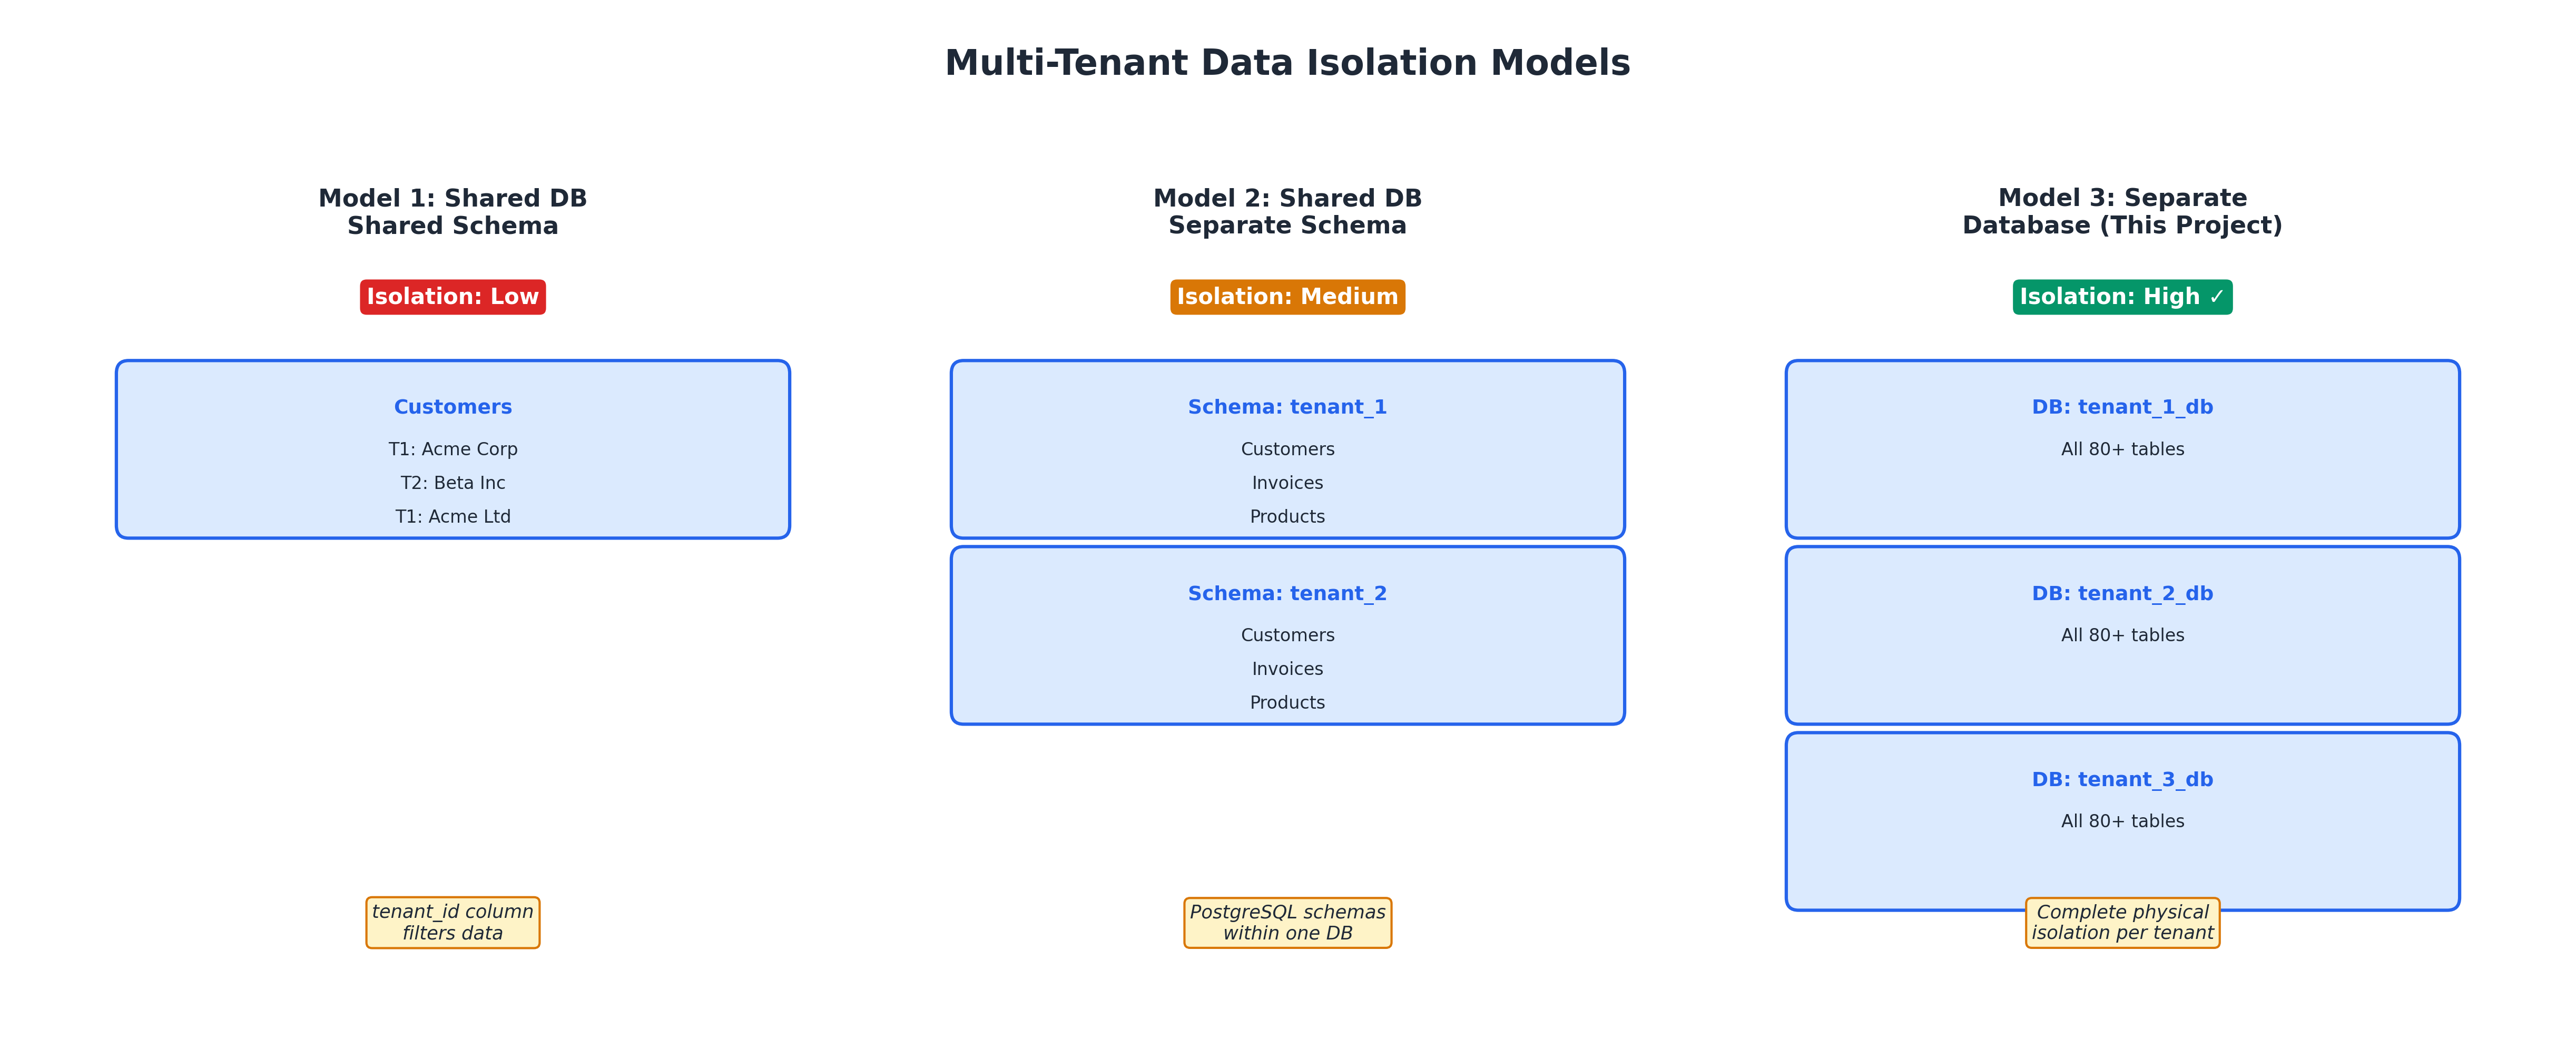
\includegraphics[width=0.95\textwidth]{figures/multi_tenancy_models.png}
    \caption{Three levels of multi-tenant data isolation}
    \label{fig:multi_tenancy_models}
\end{figure}

This project implements the \textbf{database-per-tenant} model, which provides the highest level of data isolation. Each tenant organization receives a dedicated PostgreSQL database that is dynamically provisioned via Docker containers or remote server connections. Django's database routing mechanism (\texttt{DATABASE\_ROUTERS}) is used to direct queries to the appropriate tenant database based on the authenticated user's session context.

\subsection{Multi-Tenancy in Django}

Django's built-in support for multiple databases, combined with custom database routers, makes it well-suited for implementing multi-tenant architectures. The key components in this project's implementation are:

\begin{itemize}
  \item \texttt{TenantDatabase} model: Stores connection parameters for each tenant's PostgreSQL database.
  \item \texttt{DatabaseAssignment} model: Maps users to tenant databases with role-based permissions.
  \item \texttt{add\_tenant\_database()}: Dynamically registers tenant database configurations in Django's \texttt{DATABASES} setting at runtime.
  \item \texttt{TenantDatabaseContext}: A context manager that sets the active database alias for the current thread, ensuring all ORM queries route to the correct tenant database.
  \item Custom middleware: Resolves the authenticated user's tenant database on each request and activates the appropriate database context.
\end{itemize}


\section{Machine Learning in Enterprise Systems}
\label{sec:ml_enterprise}

\subsection{Overview of ML in Business Applications}

The application of machine learning to business processes has accelerated significantly with the availability of large transactional datasets, affordable computing power, and mature ML frameworks. \citet{davenport2018ai} identify three levels of AI integration in business systems:

\begin{enumerate}[label=\arabic*.]
  \item \textbf{Process Automation:} Using ML for routine tasks such as document classification, data entry validation, and alert generation.
  \item \textbf{Cognitive Insight:} Applying ML algorithms to detect patterns in large datasets---such as customer segmentation, fraud detection, and demand forecasting---that would be impractical for human analysts.
  \item \textbf{Cognitive Engagement:} Deploying conversational AI and recommendation systems that interact directly with users, such as chatbots and personalized marketing engines.
\end{enumerate}

This project primarily operates at the \textbf{Cognitive Insight} level, embedding ML models that analyze transactional data and surface actionable insights to business users through the AI Insight Engine.

\subsection{Lead Scoring with Logistic Regression}

Lead scoring is the process of assigning a numerical value to each sales lead to predict the likelihood of conversion. \citet{provost2013data} describe logistic regression as particularly well-suited for lead scoring because it provides calibrated probability estimates (not just classifications), is inherently interpretable, and performs well with moderate-sized datasets.

In this project, the Lead Scoring model uses features including estimated deal value, lead age, activity count, lead source, and customer contact completeness. The model is trained on historical won/lost leads and outputs a conversion probability between 0 and 1.

\subsection{Payment Risk Prediction with Gradient Boosting}

Predicting whether an invoice will be paid late is a critical capability for accounts receivable management. \citet{chen2016xgboost} demonstrate that gradient boosted decision trees consistently outperform other classifiers on structured/tabular data tasks, making them ideal for invoice-level payment risk prediction.

The project's Late Payment Predictor uses 10 engineered features, including invoice amount, days to due date, customer historical payment delay, and customer type. Leave-one-out temporal statistics are used to prevent data leakage---a common pitfall identified by \citet{provost2013data} in churn and payment prediction models.

\subsection{Employee Attrition Prediction with Random Forest}

Employee turnover is costly, with the Society for Human Resource Management estimating replacement costs at 50--200\% of annual salary \citep{shrm2022}. \citet{breiman2001random} introduced Random Forest---an ensemble of decision trees trained on bootstrap samples---which has become a standard approach for employee attrition prediction due to its robustness to noisy features and native feature importance ranking.

This project's Attrition Predictor uses 10 features including tenure, salary relative to department average, leave frequency, attendance rate, and overtime hours. Class imbalance (typically fewer departures than retentions) is addressed using the \texttt{class\_weight='balanced'} parameter.

\subsection{Anomaly Detection with Isolation Forest}

\citet{liu2008isolation} proposed the Isolation Forest algorithm based on the principle that anomalies are ``few and different''---they require fewer random partitions to isolate than normal observations. This makes Isolation Forest computationally efficient and effective for unsupervised anomaly detection in expense claim analysis, where labeled fraud data is typically unavailable.

The project's Expense Anomaly Detector applies Isolation Forest with a \texttt{contamination} parameter of 0.03 (expecting 3\% of expenses to be anomalous) to features including expense amount, category, day of week, and month.

\subsection{Time-Series Forecasting with Prophet}

Facebook Prophet, introduced by \citet{taylor2018forecasting}, is an additive regression model designed for business time-series data with strong seasonal patterns and missing data points. Prophet decomposes the forecast into trend, seasonality (weekly, yearly, custom), and holiday components using a Bayesian framework.

The project uses Prophet for per-product demand forecasting, with custom monthly seasonality ($fourier\_order = 3$) and calibrated changepoint detection ($changepoint\_prior\_scale = 0.15$). Model accuracy is evaluated using Prophet's built-in cross-validation framework, achieving an average accuracy of 0.7249 across 80 product-warehouse combinations.

\subsection{Statistical Process Control for KPI Monitoring}

Z-score-based anomaly detection is a classical statistical quality control technique introduced by \citet{shewhart1931economic} and widely used in manufacturing as Shewhart control charts. When applied to business KPIs, the method flags values that deviate more than a specified number of standard deviations from the historical mean.

The project's KPI Anomaly Detector monitors five daily metrics (revenue, expenses, new leads, overdue invoices, inventory movements) against 90-day rolling baselines, generating WARNING alerts for deviations exceeding $2\sigma$ and CRITICAL alerts for deviations exceeding $3\sigma$.


\section{Related Work}
\label{sec:related_work}

\subsection{AI-Enhanced ERP Systems}

\citet{lee2020erp} survey the integration of AI technologies into ERP systems and identify three implementation strategies: (1)~embedded AI within the ERP platform itself, (2)~AI as an external service integrated via APIs, and (3)~AI as a middleware layer between the ERP and a BI platform. They conclude that the embedded approach provides the tightest integration and lowest latency but requires the deepest technical expertise. This project follows the embedded approach.

SAP introduced ``SAP Business AI'' in 2023, incorporating predictive analytics and natural language processing into S/4HANA Cloud. However, these capabilities are available only in the Enterprise tier, which carries substantial licensing costs. Oracle Fusion Cloud ERP similarly offers ML-driven anomaly detection and forecasting features in its premium offerings. No open-source ERP system currently provides comparable embedded ML capabilities.

\subsection{Multi-Tenant Django Applications}

The \texttt{django-tenants} library implements PostgreSQL schema-based multi-tenancy for Django, providing automatic schema routing via the \texttt{search\_path} mechanism. While this approach is well-tested, it does not support database-per-tenant isolation, which this project requires for maximum data separation. The \texttt{django-db-multitenant} library offers a middleware-based approach but is limited to schema-based or connection-string routing. This project implements a custom multi-tenant framework with dynamic database registration, Docker-based provisioning, and a user approval workflow---features not provided by existing libraries.

\subsection{ML for Demand Forecasting in Supply Chain}

\citet{fildes2022forecasting} provide a comprehensive review of ML approaches for retail demand forecasting, comparing classical time-series methods (ARIMA, Exponential Smoothing) with machine learning methods (Random Forest, Gradient Boosting, Neural Networks) and hybrid approaches. They find that Prophet performs competitively on datasets with strong seasonality and limited history, making it well-suited for SME inventory data where per-product histories may span only 6--12 months.


\section{Gap Analysis}
\label{sec:gap_analysis}

The literature review reveals the following gaps that this project addresses:

\begin{table}[H]
\centering
\caption{Literature gap analysis and project contributions}
\label{tab:gap_analysis}
\begin{tabularx}{\textwidth}{>{\raggedright\arraybackslash}X >{\raggedright\arraybackslash}X >{\raggedright\arraybackslash}X}
\toprule
\textbf{Gap Identified} & \textbf{Supporting Literature} & \textbf{Project Contribution} \\
\midrule
No open-source ERP with embedded ML & \citet{lee2020erp}; SAP/Oracle features are premium-only & 8 ML models embedded in a free, open-source ERP \\
\addlinespace
Limited multi-tenant options in Django & django-tenants supports schema-only; django-db-multitenant lacks provisioning & Custom DB-per-tenant with Docker provisioning and role-based access \\
\addlinespace
Poor Arabic support in open-source ERP & \citet{alkraiji2020}; Odoo/ERPNext have partial translations & Dual-language fields (\texttt{name}/\texttt{name\_ar}) in 80+ models \\
\addlinespace
ML models disconnected from ERP workflow & Most ML-ERP integrations use external BI tools & Inline ML training, prediction logging, and AI Insight notifications \\
\addlinespace
Lack of cross-domain ML in single ERP & Studies focus on single domains (finance OR HR OR supply chain) & Models span CRM, Finance, HR, Inventory, and Operations \\
\bottomrule
\end{tabularx}
\end{table}

\section{Summary}
\label{sec:lit_summary}

This chapter reviewed the evolution and current state of ERP systems, multi-tenant software architectures, and the application of machine learning in enterprise settings. The review established that while commercial ERP vendors have begun incorporating AI capabilities, these features remain inaccessible to SMEs due to cost and complexity. Open-source ERP alternatives lack both native multi-tenancy and integrated ML. This project bridges these gaps by combining a production-quality multi-tenant ERP with eight embedded ML models, delivered through an Agile Sprint development process that is detailed in the following chapter.


% ██████████████████████████████████████████████████████████████████
%
%  CHAPTER 3 — METHODOLOGY
%
% ██████████████████████████████████████████████████████████████████
\chapter{Methodology}
\label{ch:methodology}

\section{Introduction}
\label{sec:meth_intro}

This chapter presents the development methodology, system architecture, technology stack, data collection approach, and machine learning pipeline design adopted for this project. The Sprint (Agile) methodology was selected as the software development lifecycle (SDLC) model to accommodate the project's complexity, evolving requirements, and the iterative nature of ML model development.

\section{Development Methodology: Sprint (Agile)}
\label{sec:sprint_methodology}

\subsection{Overview of Sprint Methodology}

The Sprint methodology, as defined in the Scrum framework \citep{schwaber2020scrum}, organizes software development into fixed-length iterations called \textbf{Sprints}, typically lasting 1--4 weeks. Each Sprint follows a structured cycle: planning, development, testing, review, and retrospective. This iterative approach is particularly well-suited for projects with complex, multi-module architectures and evolving requirements---both characteristics of this ERP system.

\begin{figure}[H]
    \centering
    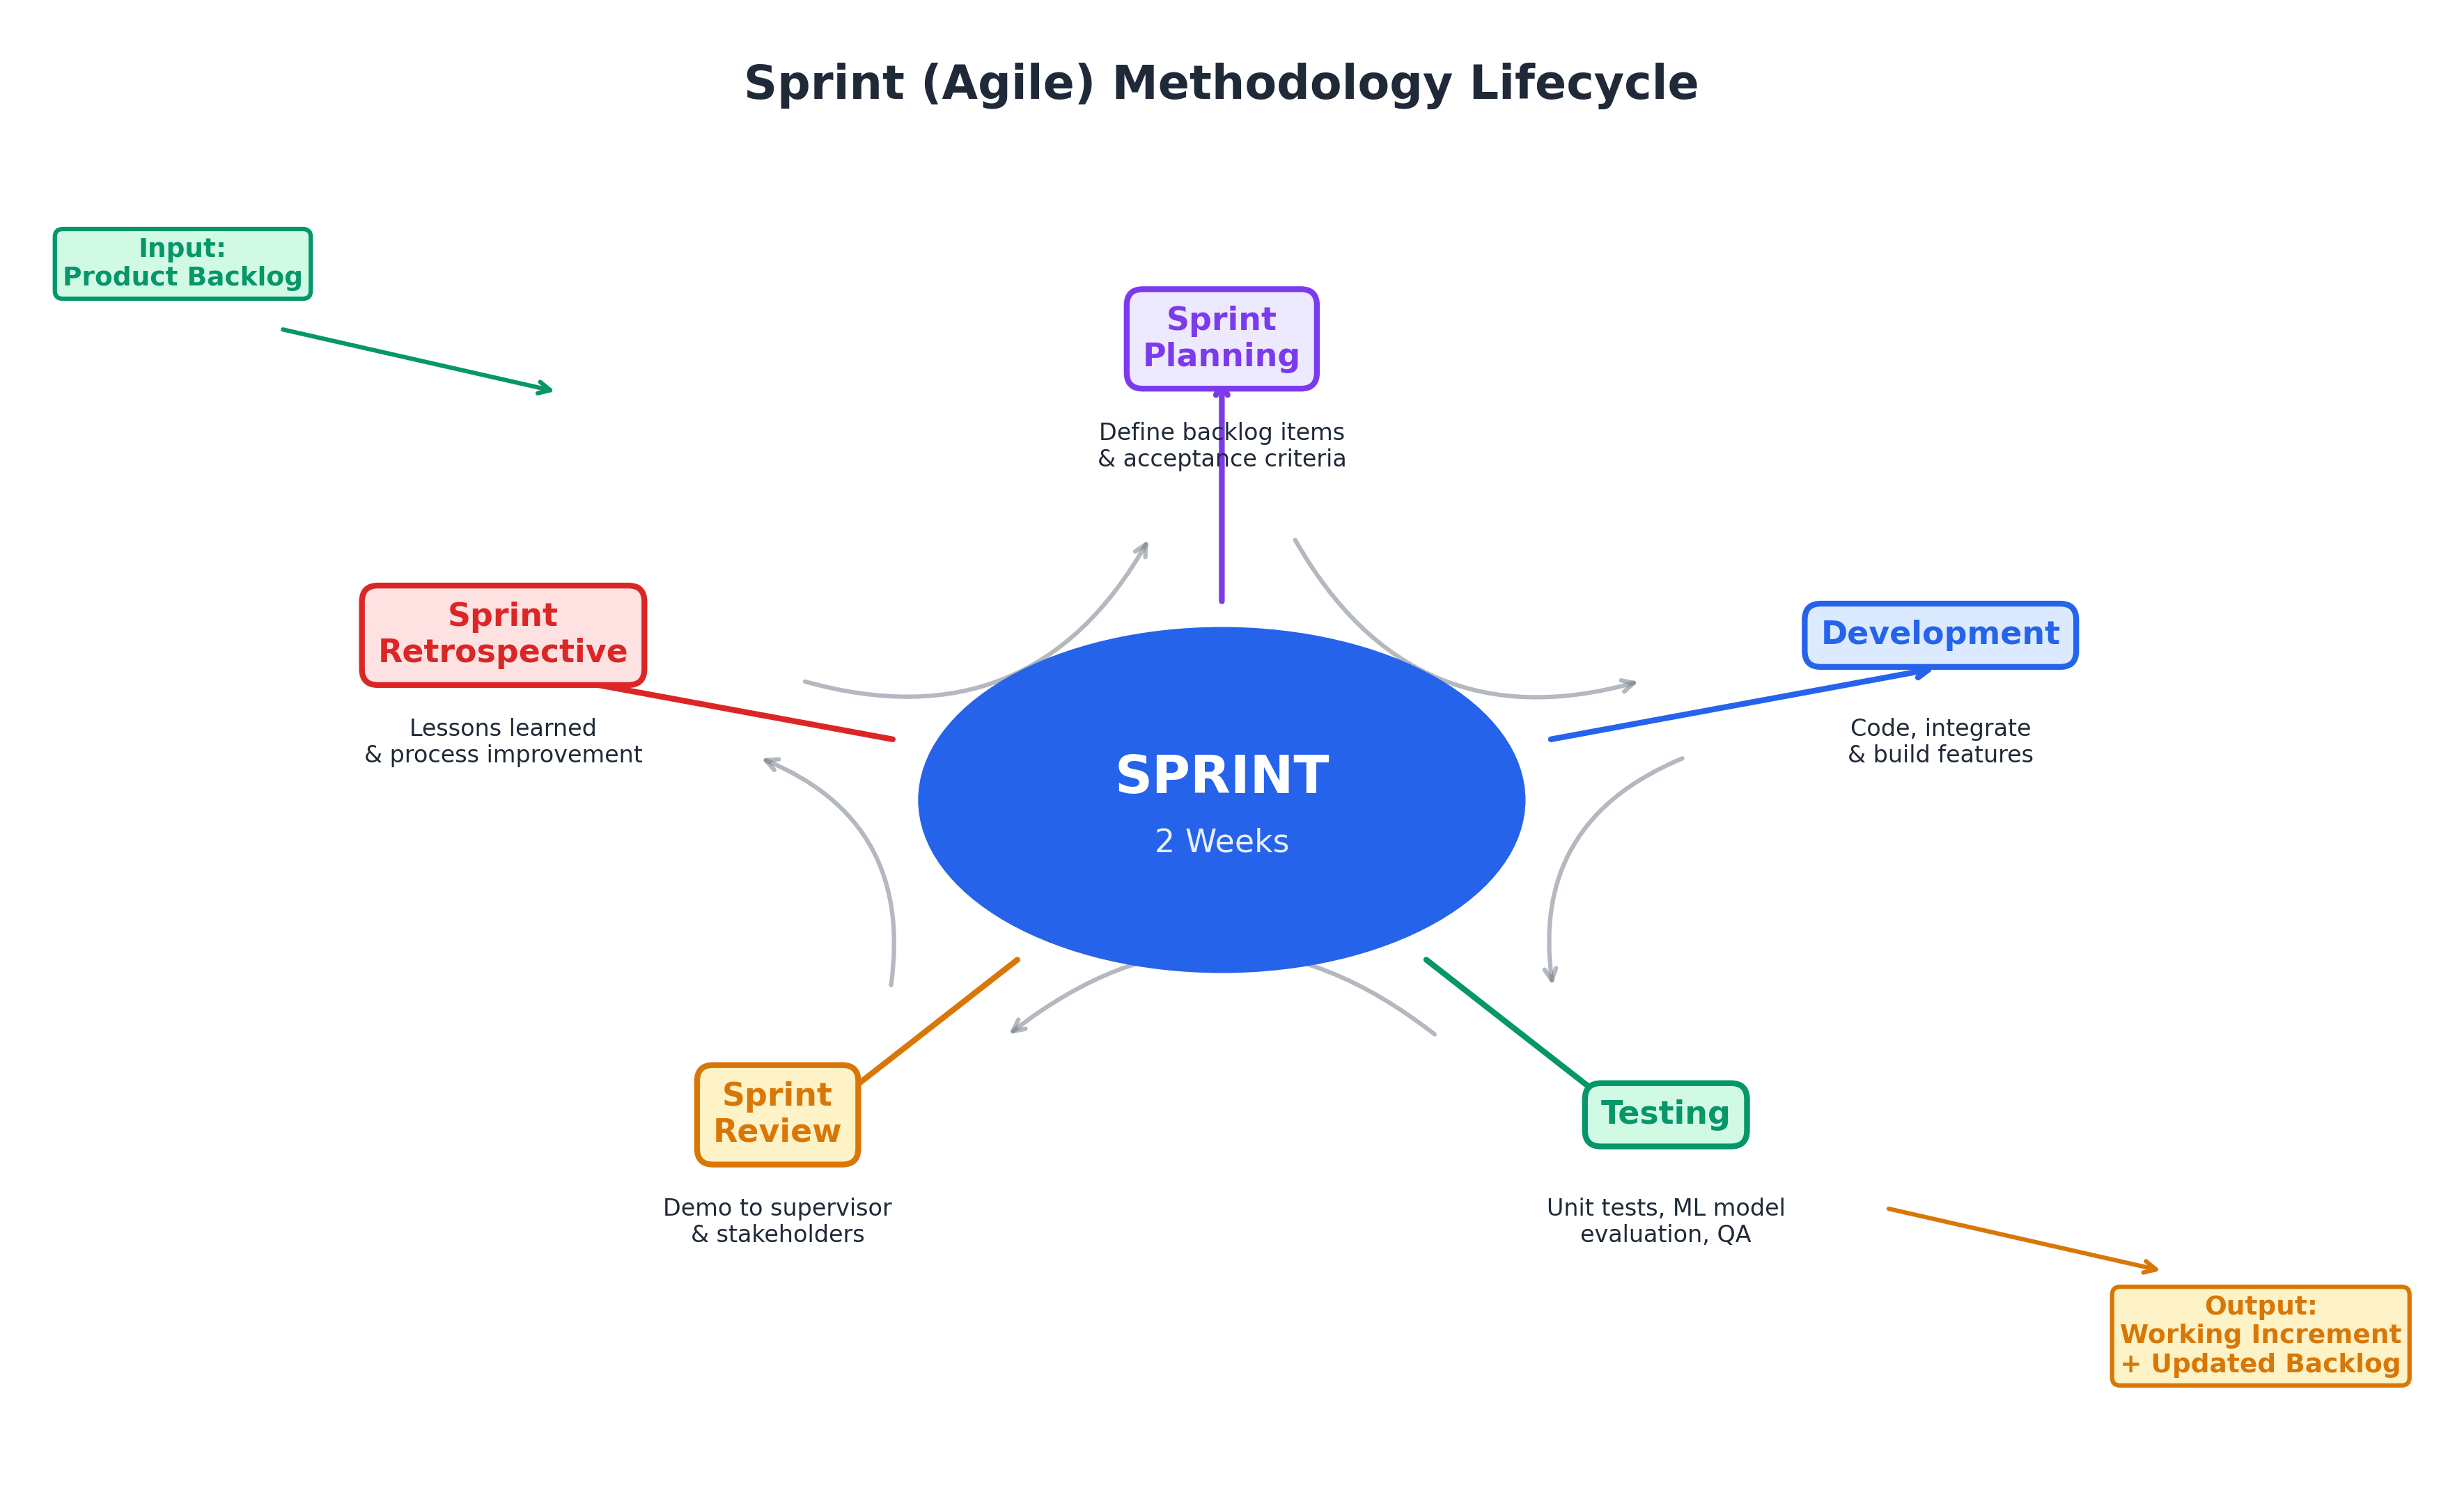
\includegraphics[width=0.85\textwidth]{figures/sprint_lifecycle.png}
    \caption{Sprint (Agile) methodology lifecycle}
    \label{fig:sprint_lifecycle}
\end{figure}

The key principles of the Sprint methodology applied to this project include:

\begin{itemize}
  \item \textbf{Iterative Delivery:} Each Sprint produces a working increment of the system, allowing stakeholders to review functional modules progressively rather than waiting for a final monolithic delivery.

  \item \textbf{Adaptive Planning:} Sprint planning sessions at the beginning of each iteration allow the team to reprioritize tasks based on feedback, discovered dependencies, and technical challenges.

  \item \textbf{Continuous Integration and Testing:} Code is tested at the end of each Sprint, including unit tests for ML model accuracy and integration tests for API endpoints.

  \item \textbf{Feedback-Driven Improvement:} Sprint retrospectives identify process improvements, while Sprint reviews validate that delivered features meet acceptance criteria.
\end{itemize}

\subsection{Sprint Plan for This Project}

The project was organized into \textbf{seven Sprints} over the development period. Table~\ref{tab:sprint_plan} summarizes the Sprint plan:

\begin{table}[H]
\centering
\caption{Sprint plan and deliverables}
\label{tab:sprint_plan}
\begin{tabularx}{\textwidth}{c c >{\raggedright\arraybackslash}X >{\raggedright\arraybackslash}X}
\toprule
\textbf{Sprint} & \textbf{Duration} & \textbf{Focus Area} & \textbf{Deliverables} \\
\midrule
1 & 2 weeks & Project Setup \& Multi-Tenant Architecture & Django project scaffold, TenantUser model, PostgresServer model, TenantDatabase model, database routing, user approval workflow \\
\addlinespace
2 & 2 weeks & Core ERP Modules (Finance \& HR) & Company, Currency, Department, Employee, Attendance, Payroll, Invoice, Payment, Expense, Chart of Accounts \\
\addlinespace
3 & 2 weeks & CRM, Supplier \& Procurement & Lead, LeadActivity, Campaign, Customer, Supplier, PurchaseOrder, SupplierInvoice, SupplierPayment \\
\addlinespace
4 & 2 weeks & Inventory/WMS \& POS & Warehouse, zones/bins, StockMovement, GoodsReceipt, StockTransfer, CycleCount, PickList, ShipmentNote, ReorderRule, POS terminal/session/order \\
\addlinespace
5 & 2 weeks & ML Model Development & AI model registry, 8 ML service modules, training pipeline, prediction logging, AI Insight engine \\
\addlinespace
6 & 2 weeks & Data Integration \& ML Tuning & Dataset import commands, synthetic data seeding, Prophet hyperparameter tuning, KPI calibration, model evaluation \\
\addlinespace
7 & 2 weeks & Testing, Documentation \& Deployment & Integration testing, API documentation, deployment configuration (Gunicorn + Docker), thesis writing \\
\bottomrule
\end{tabularx}
\end{table}

\begin{figure}[H]
    \centering
    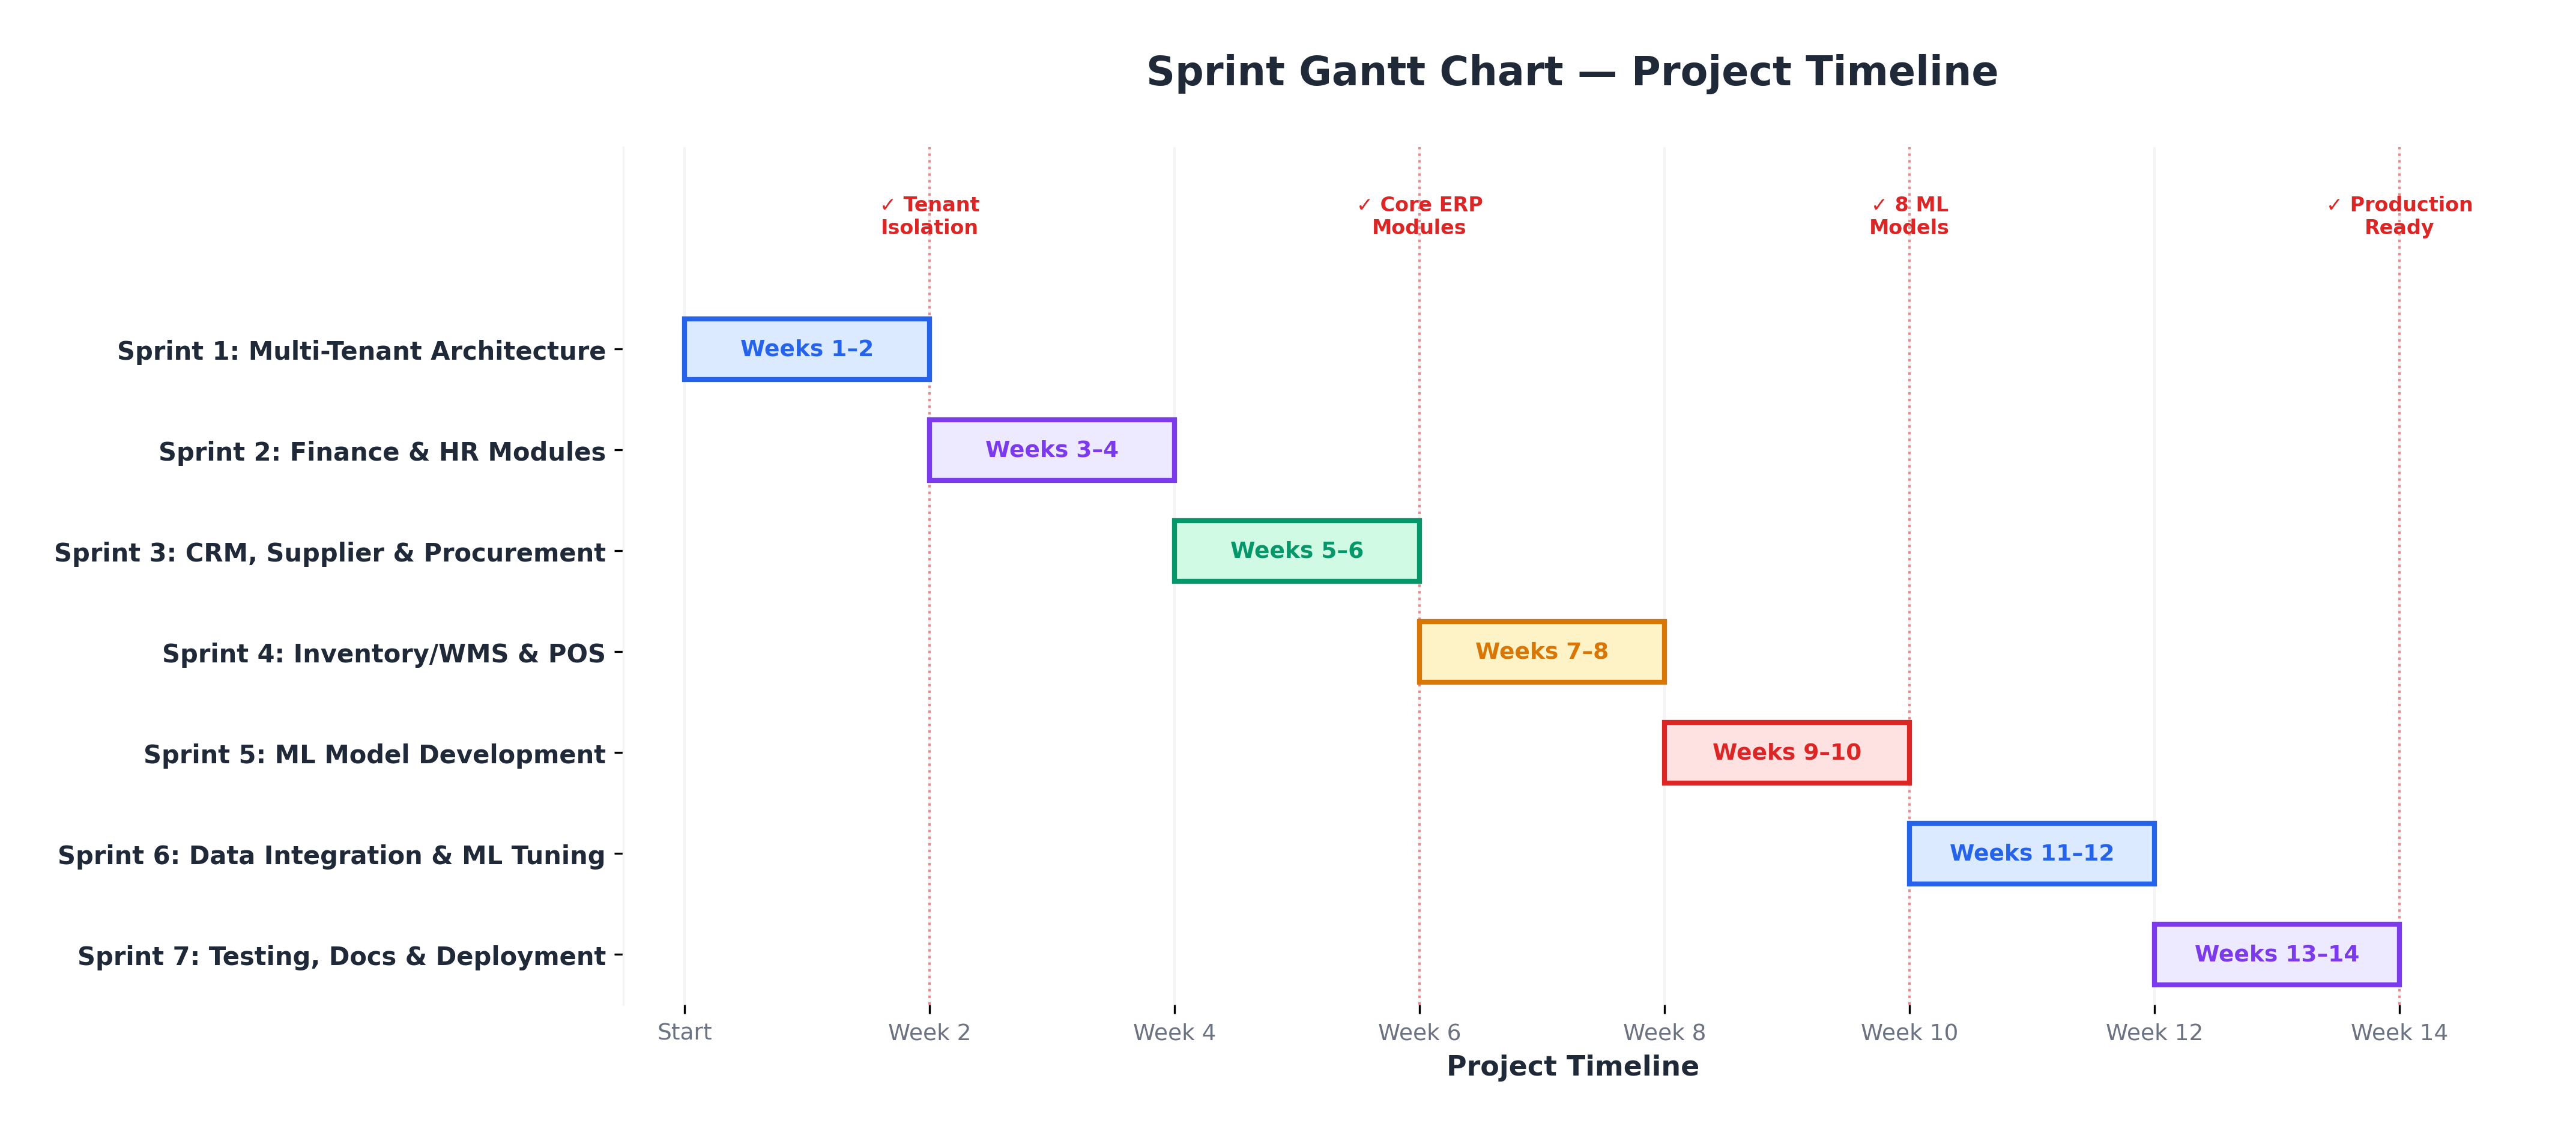
\includegraphics[width=0.95\textwidth]{figures/sprint_gantt_chart.png}
    \caption{Gantt chart showing Sprint timeline and dependencies}
    \label{fig:gantt_chart}
\end{figure}

\subsection{Sprint Roles}

Although this is an individual graduation project, the Sprint methodology roles were adapted as follows:

\begin{itemize}
  \item \textbf{Product Owner:} The project supervisor, who reviewed Sprint deliverables and provided feedback on priorities and acceptance criteria.
  \item \textbf{Scrum Master / Developer:} The student (Salah Abdullah Khalil), responsible for Sprint planning, development, testing, and retrospective documentation.
  \item \textbf{Stakeholders:} The academic committee and potential end users who provided domain feedback during the CRM, Finance, and HR module development.
\end{itemize}

\subsection{Justification for Sprint Methodology}

The Sprint methodology was chosen over alternative SDLC models for the following reasons:

\begin{table}[H]
\centering
\caption{SDLC model comparison and justification}
\label{tab:sdlc_comparison}
\begin{tabularx}{\textwidth}{l >{\raggedright\arraybackslash}X >{\raggedright\arraybackslash}X}
\toprule
\textbf{SDLC Model} & \textbf{Strengths} & \textbf{Limitation for This Project} \\
\midrule
Waterfall & Clear phases, thorough documentation & Does not accommodate changing requirements; ML models require iterative tuning \\
\addlinespace
V-Model & Strong testing emphasis & Sequential nature delays integration testing \\
\addlinespace
RAD & Rapid prototyping & Insufficient emphasis on architecture for a system with 80+ models \\
\addlinespace
\textbf{Sprint (Agile)} & Iterative delivery, accommodates ML experimentation, continuous feedback & Requires discipline in documentation (addressed through Sprint reviews) \\
\bottomrule
\end{tabularx}
\end{table}


\section{System Architecture}
\label{sec:architecture}

\subsection{High-Level Architecture}

The system follows a three-tier architecture: Presentation Layer (Django templates + REST API), Application Layer (Django views, services, and ML pipelines), and Data Layer (PostgreSQL databases with multi-tenant routing).

\begin{figure}[H]
    \centering
    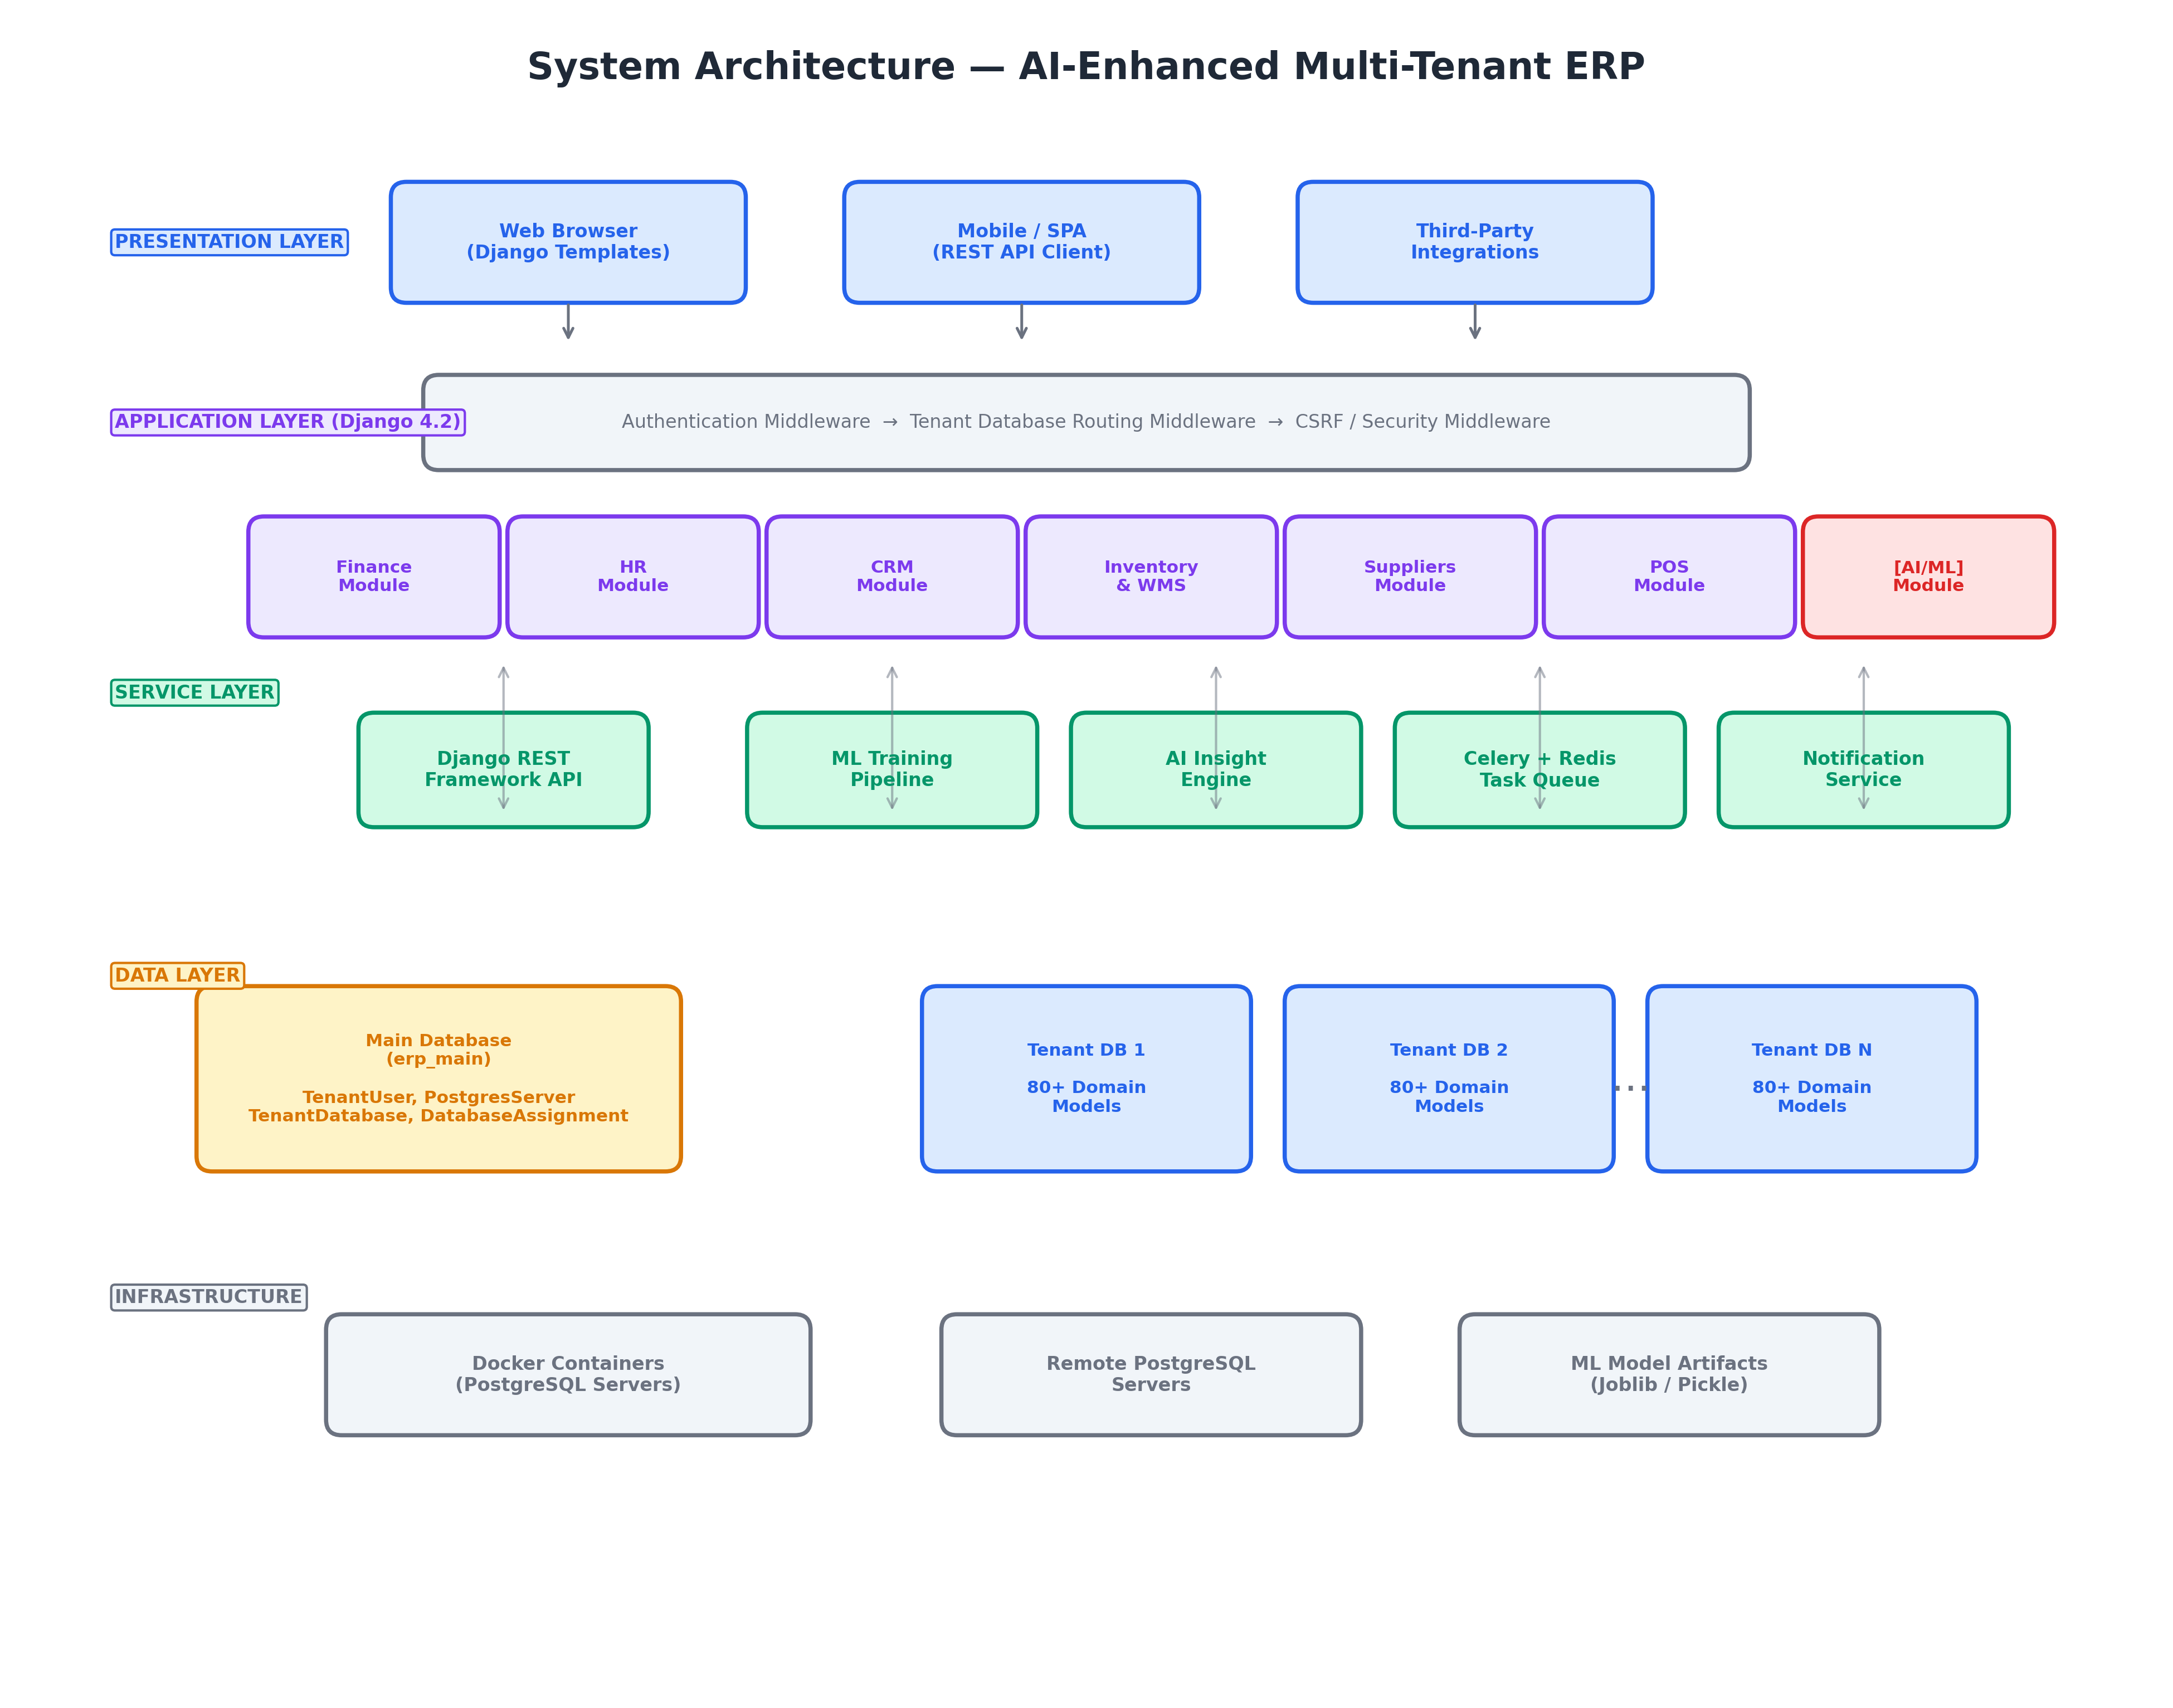
\includegraphics[width=0.95\textwidth]{figures/system_architecture.png}
    \caption{High-level system architecture showing the three-tier design with multi-tenant database routing}
    \label{fig:system_architecture}
\end{figure}

\subsection{Multi-Tenant Database Architecture}

The multi-tenant architecture is implemented using the database-per-tenant isolation model. The platform maintains a \textbf{main database} (\texttt{erp\_main}) that stores user accounts, server configurations, and tenant metadata. Each approved tenant organization receives a dedicated PostgreSQL database provisioned on a selected server (Docker container or remote server).

\begin{figure}[H]
    \centering
    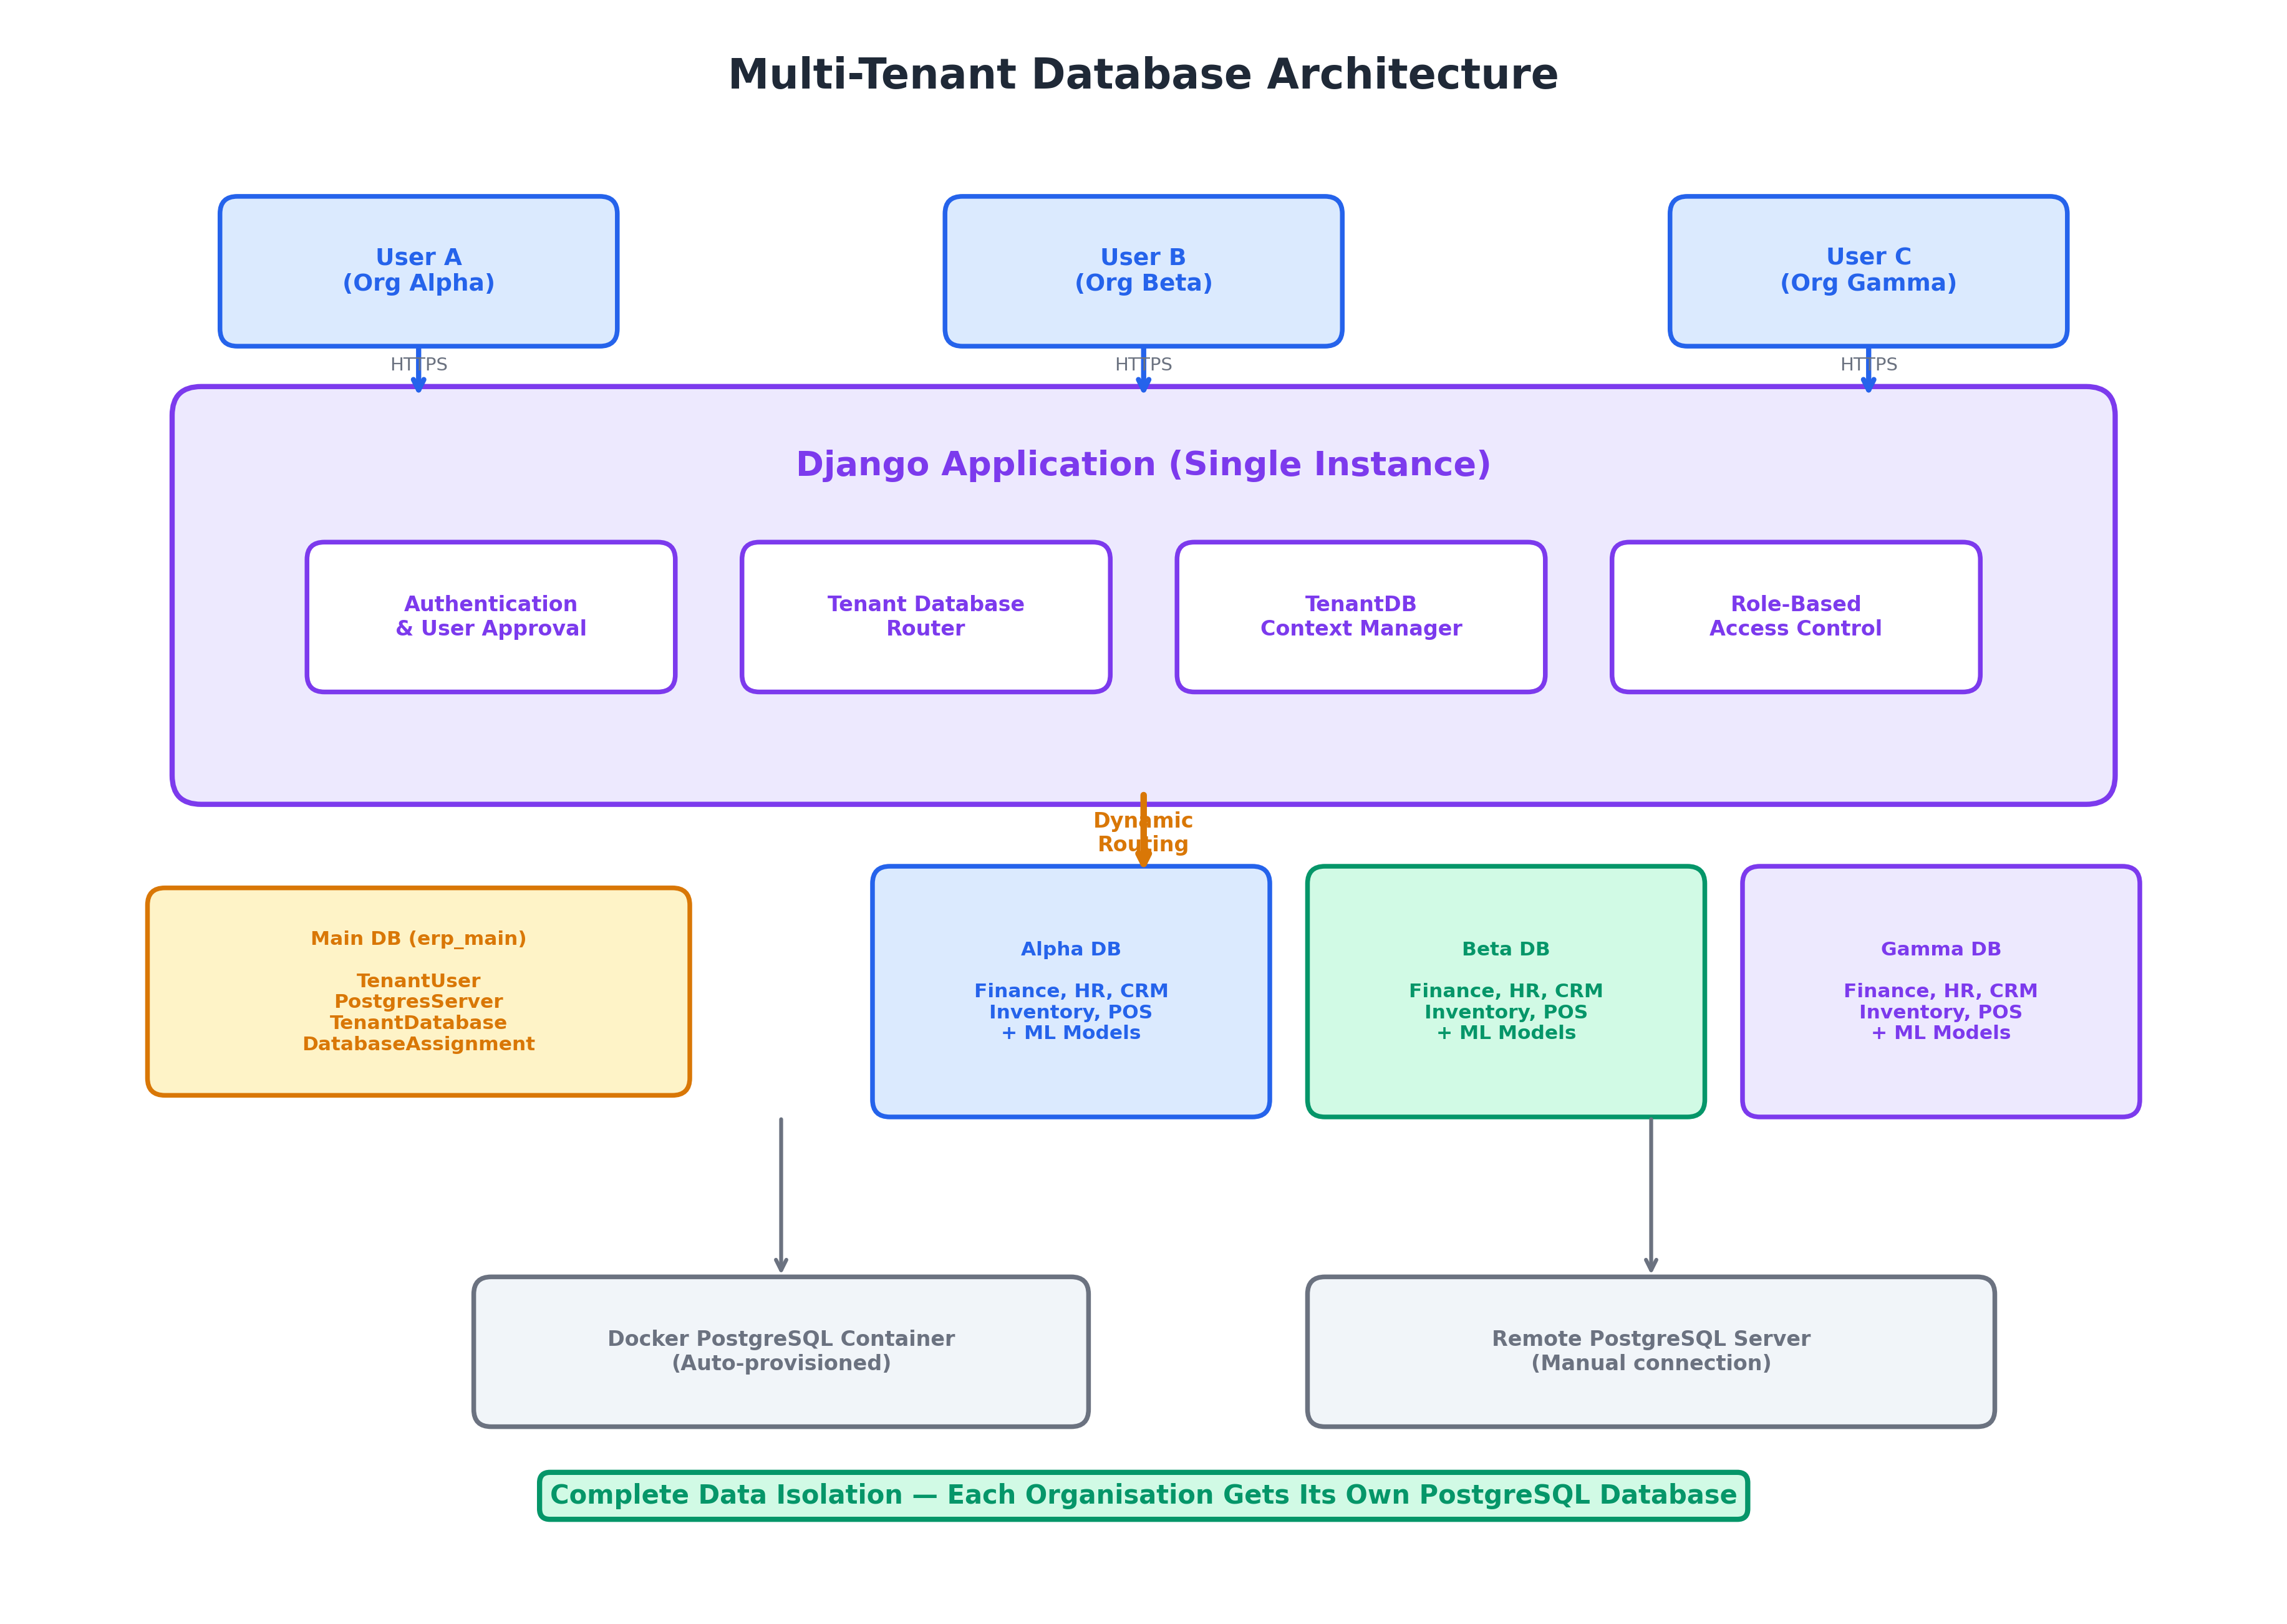
\includegraphics[width=0.95\textwidth]{figures/multi_tenant_architecture.png}
    \caption{Database-per-tenant architecture with dynamic PostgreSQL provisioning}
    \label{fig:multi_tenant_arch}
\end{figure}

The database routing mechanism works as follows:

\begin{enumerate}[label=\arabic*.]
  \item The user logs in and the authentication middleware identifies their \texttt{DatabaseAssignment}.
  \item The \texttt{add\_tenant\_database()} function dynamically registers the tenant's database connection parameters in Django's \texttt{DATABASES} dictionary.
  \item The \texttt{TenantDatabaseContext} context manager sets the active database alias for the current request thread.
  \item All subsequent ORM queries are automatically routed to the tenant's database via the custom \texttt{DATABASE\_ROUTERS} configuration.
  \item When the request completes, the context manager resets the routing.
\end{enumerate}

\subsection{AI/ML Pipeline Architecture}

The ML pipeline is integrated into the ERP as a self-contained module (\texttt{erp.ai}) with the following components:

\begin{itemize}
  \item \textbf{Model Registry} (\texttt{MLModel}): Tracks model versions, accuracy scores, training parameters, and artefact file paths. Each model is scoped to a specific company (tenant).

  \item \textbf{Service Layer} (\texttt{erp.ai.services}): Contains the implementation of each ML model as a Python class. Each service class follows a consistent interface: \texttt{train()}, \texttt{predict()}, and an optional \texttt{score\_all()} batch method.

  \item \textbf{Training Pipeline} (\texttt{train\_models} management command): An orchestrator that sequentially trains all selected models, evaluates their performance, and generates a JSON training report.

  \item \textbf{Prediction Logging} (\texttt{PredictionLog}): An immutable audit trail of every prediction made, enabling future retraining on actual outcomes.

  \item \textbf{AI Insight Engine} (\texttt{AIInsight} + \texttt{create\_or\_update\_insight}): Converts ML model outputs into human-readable alerts with severity levels, recommendations, and action URLs. Includes automatic deduplication via a configurable cooldown window.
\end{itemize}

\begin{figure}[H]
    \centering
    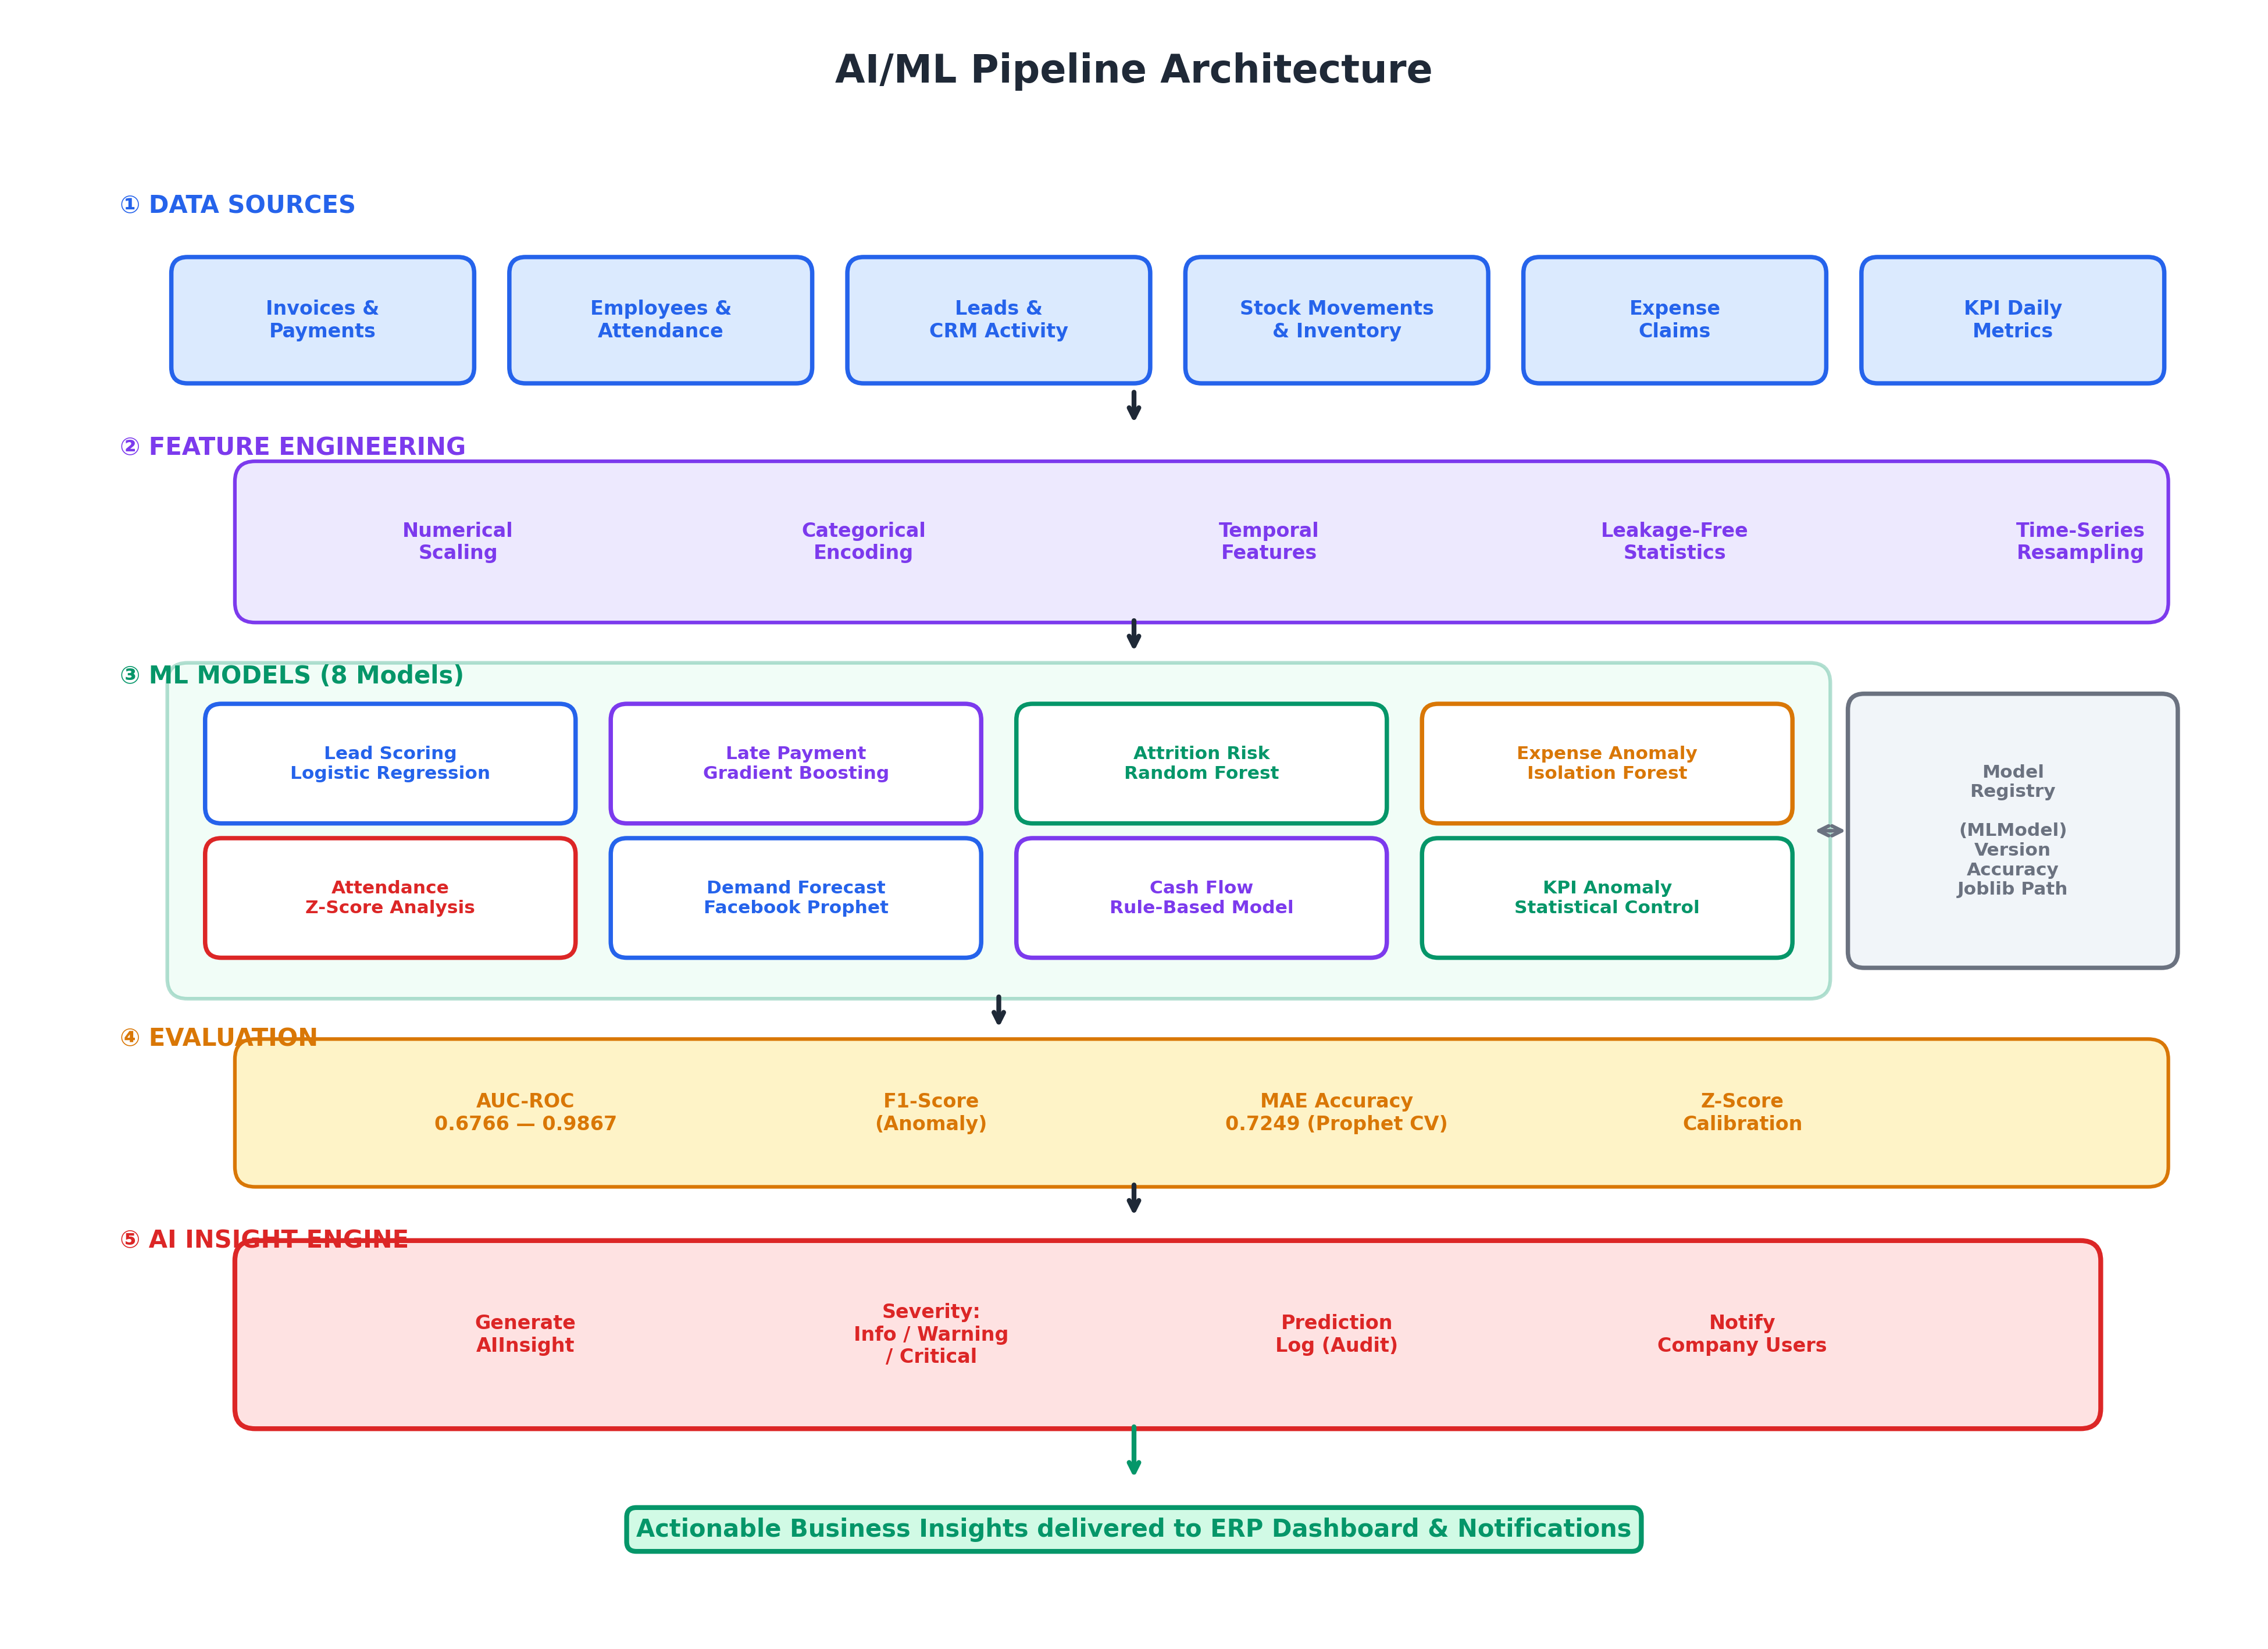
\includegraphics[width=0.95\textwidth]{figures/ml_pipeline_architecture.png}
    \caption{AI/ML pipeline architecture showing the flow from raw data to actionable insights}
    \label{fig:ml_pipeline}
\end{figure}


\section{Technology Stack}
\label{sec:tech_stack}

Table~\ref{tab:tech_stack} summarizes the technologies used in this project:

\begin{table}[H]
\centering
\caption{Technology stack}
\label{tab:tech_stack}
\begin{tabularx}{\textwidth}{l l >{\raggedright\arraybackslash}X}
\toprule
\textbf{Layer} & \textbf{Technology} & \textbf{Purpose} \\
\midrule
Backend Framework & Django 4.2 & Web framework, ORM, URL routing, template engine \\
Programming Language & Python 3.12 & Primary development language \\
Database & PostgreSQL 12+ & Relational database for main and tenant databases \\
REST API & Django REST Framework 3.14 & RESTful API layer for mobile/third-party integration \\
ML / Data Science & scikit-learn 1.4, pandas 2.0, numpy 1.26 & Classical ML algorithms and data processing \\
Time-Series Forecasting & Facebook Prophet 1.1.5 & Additive regression for demand forecasting \\
LLM Integration & OpenAI API (GPT-4o-mini) & AI assistant and natural language analysis \\
Task Queue & Celery 5.3 + Redis 5.0 & Asynchronous ML training and background jobs \\
Containerization & Docker + docker-py 6.1 & Dynamic PostgreSQL server provisioning \\
Frontend & Django Templates + Bootstrap 5 + Crispy Forms & Server-side rendered responsive UI \\
PDF Generation & xhtml2pdf 0.2 & Invoice and report PDF export \\
Data Visualization & Plotly 5.22 & Interactive charts and dashboards \\
Version Control & Git + GitHub & Source code management \\
Deployment & Gunicorn 21.2 & WSGI HTTP server for production \\
\bottomrule
\end{tabularx}
\end{table}


\section{Data Collection and Preparation}
\label{sec:data_collection}

The ML models in this project are trained on a combination of real-world open-source datasets and synthetic domain-specific data generated to fill coverage gaps:

\subsection{Open-Source Datasets}

\begin{enumerate}[label=\arabic*.]
  \item \textbf{Olist Brazilian E-Commerce Dataset} \citep{olist2018}: A public dataset from Kaggle containing over 100,000 real e-commerce orders from Brazilian marketplaces (2016--2018). This dataset provides:
  \begin{itemize}
    \item 99,441 orders with order dates, delivery dates, and payment information
    \item 32,216 products across 73 categories
    \item 96,096 customers with geolocation data
    \item 3,095 sellers
  \end{itemize}
  The Olist dataset was used to populate the Customers, Products, Invoices, Orders, and Payments modules.

  \item \textbf{IBM HR Employee Attrition Dataset} \citep{ibm2017hr}: A synthetic but statistically realistic dataset of 1,470 employee records with 35 attributes including salary, department, overtime hours, and attrition labels. This dataset trains the Employee Attrition Prediction model.

  \item \textbf{Supplier Procurement Dataset}: A custom-generated dataset of 50 suppliers and 873 purchase orders with realistic procurement cycles, used to populate the Supplier and Purchase Order modules.

  \item \textbf{Attendance Timeseries Dataset}: A custom-generated dataset of employee attendance records spanning 12 months with check-in/check-out times, hours worked, late arrival flags, and overtime hours.

  \item \textbf{Expense Claims Dataset}: A custom-generated dataset of 6,278 approved expense claims with embedded anomalies (labeled \texttt{is\_anomaly} column) for Isolation Forest evaluation.

  \item \textbf{CRM Leads Dataset}: A custom-generated dataset of 4,062 leads with source, estimated value, activities, and won/lost outcomes.
\end{enumerate}

\subsection{Synthetic Data Generation}

For modules without corresponding real-world datasets---particularly Inventory/WMS and KPI monitoring---a data seeding utility (\texttt{seed\_ml\_operational\_data}) was developed. This management command generates:

\begin{itemize}
  \item \textbf{Stock Movements:} 365 days of daily demand history for 80 products with weekly and monthly seasonality, product diversity profiles (fast/moderate/slow movers), weekend dips, growth trends, and random noise.

  \item \textbf{Reorder Rules:} 80 product-warehouse rule configurations with randomized lead times, safety stock levels, and minimum order quantities.

  \item \textbf{Supplier Invoices:} 220 pending supplier invoices with due dates spanning the next 90 days for Cash Flow projection.

  \item \textbf{KPI Spike Injection:} Calibrated inventory movement spikes targeting z-score $\approx 3.5\sigma$ above the 90-day baseline for KPI Anomaly Detection testing.
\end{itemize}


\section{Machine Learning Model Design}
\label{sec:ml_design}

\subsection{Model Selection Criteria}

The ML models were selected based on four criteria:

\begin{enumerate}[label=\arabic*.]
  \item \textbf{Interpretability:} Business users must understand why a prediction was made. Models with native feature importance (Random Forest, Gradient Boosting) and calibrated probabilities (Logistic Regression) were preferred.

  \item \textbf{Data Efficiency:} SME datasets are typically small (hundreds to low thousands of records). Models that perform well with limited data (Prophet, Z-Score, Isolation Forest) were favored.

  \item \textbf{Operational Simplicity:} Models must train in seconds to minutes on a standard server, serialize as compact files (joblib), and produce predictions with sub-second latency.

  \item \textbf{Task Appropriateness:} Each algorithm was matched to its problem type---classification (Logistic Regression, GBM, Random Forest), unsupervised anomaly detection (Isolation Forest, Z-Score), time-series forecasting (Prophet), and rule-based projection (Cash Flow).
\end{enumerate}

\subsection{Model Specifications}

Table~\ref{tab:ml_models} summarizes the eight ML models implemented in this project:

\begin{longtable}{p{2.5cm} p{2cm} p{2.5cm} p{2.5cm} p{2cm} p{1.5cm}}
\caption{ML model specifications} \label{tab:ml_models} \\
\toprule
\textbf{Model} & \textbf{Domain} & \textbf{Algorithm} & \textbf{Features} & \textbf{Evaluation Metric} & \textbf{Min. Samples} \\
\midrule
\endfirsthead
\caption[]{ML model specifications (continued)} \\
\toprule
\textbf{Model} & \textbf{Domain} & \textbf{Algorithm} & \textbf{Features} & \textbf{Evaluation Metric} & \textbf{Min. Samples} \\
\midrule
\endhead
Lead Scoring & CRM & Logistic Regression (C=1.0) & 7 features (value, age, activities, source, contact info) & AUC-ROC & 30 \\
\addlinespace
Late Payment & Finance & Gradient Boosting (300 trees, depth=5, lr=0.08) & 10 features (amount, days-to-due, customer history) & AUC-ROC & 30 \\
\addlinespace
Attrition & HR & Random Forest (300 trees, depth=8, balanced) & 10 features (tenure, salary, attendance, overtime) & AUC-ROC & 30 \\
\addlinespace
Expense Anomaly & Finance & Isolation Forest (300 trees, contamination=3\%) & 4 features (amount, month, weekday, category) & F1-Score vs. ground truth & 30 \\
\addlinespace
Attendance Anomaly & HR & Z-Score (threshold=2.0) & 2 metrics (avg hours, late arrival ratio) & Anomaly count & 1 \\
\addlinespace
Demand Forecast & Inventory & Prophet (additive, weekly + monthly seasonality) & Daily demand history per product/warehouse & MAE-based accuracy via cross-validation & 30 \\
\addlinespace
Cash Flow & Finance & Rule-based (30/60/90-day projection) & Outstanding invoices + pending payables + open POs & Net cash position & 0 \\
\addlinespace
KPI Anomaly & Operations & Z-Score (threshold $\geq 2\sigma$ warning, $\geq 3\sigma$ critical) & 5 daily KPIs (revenue, expenses, leads, overdue invoices, inventory movements) & Alert accuracy & 14 \\
\bottomrule
\end{longtable}

\subsection{Model Evaluation Strategy}

Each model is evaluated using appropriate metrics for its task type:

\begin{itemize}
  \item \textbf{Classifiers} (Lead Scoring, Late Payment, Attrition): AUC-ROC on a stratified 80/20 train/test split. AUC-ROC is preferred over accuracy because the datasets exhibit class imbalance.

  \item \textbf{Anomaly Detectors} (Expense Anomaly): Precision, Recall, and F1-Score computed against a ground-truth \texttt{is\_anomaly} label in the expense dataset.

  \item \textbf{Time-Series Forecasts} (Demand): MAE-based accuracy ($1 - \frac{MAE}{\bar{y}}$) computed via Prophet's built-in cross-validation with expanding windows.

  \item \textbf{Statistical Detectors} (Attendance Anomaly, KPI Anomaly): Qualitative evaluation based on the number of alerts generated and their clinical reasonableness (e.g., z-score magnitude aligning with injected anomalies).

  \item \textbf{Cash Flow}: Validation against known payables and receivables in the database---checking that inflows equal outstanding invoice balances and outflows match pending supplier invoices.
\end{itemize}


\section{Development Tools and Environment}
\label{sec:dev_tools}

\begin{table}[H]
\centering
\caption{Development tools and environment}
\label{tab:dev_tools}
\begin{tabularx}{\textwidth}{l l >{\raggedright\arraybackslash}X}
\toprule
\textbf{Category} & \textbf{Tool} & \textbf{Purpose} \\
\midrule
IDE & Visual Studio Code & Primary code editor with Python and Django extensions \\
AI Pair Programming & GitHub Copilot (Claude) & AI-assisted code generation and debugging \\
Version Control & Git + GitHub & Source code management and collaboration \\
Database Client & pgAdmin 4 & PostgreSQL database management and querying \\
API Testing & Django REST Framework browsable API & Interactive API testing and documentation \\
Virtual Environment & Python venv & Dependency isolation \\
Operating System & Windows 11 & Development machine OS \\
Browser & Google Chrome DevTools & Frontend debugging and responsive design testing \\
\bottomrule
\end{tabularx}
\end{table}


\section{Summary}
\label{sec:meth_summary}

This chapter detailed the Sprint (Agile) methodology adopted for the project, breaking the development into seven two-week Sprints covering platform architecture through ML tuning and deployment. The three-tier system architecture with database-per-tenant multi-tenancy was described, along with the AI/ML pipeline that trains, evaluates, logs, and surfaces model outputs as actionable business insights. The technology stack centers on Django 4.2, PostgreSQL, scikit-learn, and Facebook Prophet. Data collection combines six real-world and synthetic datasets totaling over 140,000 records across five business domains. The following chapter presents the detailed system analysis and design, including use case diagrams, class diagrams, and database schema design.


% ══════════════════════════════════════════════════════════════════
%  BIBLIOGRAPHY
% ══════════════════════════════════════════════════════════════════
\bibliographystyle{apalike}
\bibliography{references}

\end{document}
